\documentclass[11pt]{article}

% ---------------------------------------------------------------
% Adapting the actor model of concurrency to hybrid CPU/FPGA architectures
% Companion to arXiv:2609.21173.
% arXiv preprint --- primary cs.DC; cross-list cs.AR, q-fin.TR
% ---------------------------------------------------------------

\usepackage[utf8]{inputenc}
\usepackage[T1]{fontenc}
\usepackage{lmodern}
\usepackage{amsmath,amssymb}
\usepackage{booktabs}
\usepackage{geometry}
\usepackage{hyperref}
\usepackage{xcolor}
\usepackage{enumitem}
\usepackage{microtype}
\usepackage{caption}
\captionsetup{font=small, labelfont=bf, labelsep=period}
\usepackage{placeins}
\usepackage{graphicx}
\usepackage{listings}
\lstset{language=C++, basicstyle=\ttfamily\footnotesize, columns=fullflexible,
  keepspaces=true, frame=single, framerule=0.3pt, rulecolor=\color{gray!60},
  xleftmargin=4pt, xrightmargin=4pt, aboveskip=6pt, belowskip=6pt,
  keywordstyle=\bfseries, commentstyle=\itshape\color{gray!80!black},
  showstringspaces=false, breaklines=true}
\usepackage[text={DRAFT},color={[gray]{0.88}},scale=1.2,angle=45]{draftwatermark}
\renewcommand{\topfraction}{0.9}
\renewcommand{\bottomfraction}{0.8}
\renewcommand{\textfraction}{0.07}
\renewcommand{\floatpagefraction}{0.75}
\setcounter{topnumber}{3}
\setcounter{bottomnumber}{2}
\setcounter{totalnumber}{5}
\geometry{margin=1in}
\hypersetup{colorlinks=true, linkcolor=blue!50!black, citecolor=blue!50!black,
            urlcolor=blue!50!black}
\graphicspath{{img/fpga/}}

\newcommand{\fs}{\texttt{fast\_send}}
\newcommand{\snd}{\texttt{send}}

\title{\textbf{Adapting the Actor Model of Concurrency to\\
Hybrid CPU/FPGA Architectures}\\
\large FPGA Actors, CPU--FPGA Messaging over PCIe, and a Market-Data Handler
Without a Decode Tail}

\author{%
  Vincent Maciejewski\\
  \small M2 Technologies\\
  \small \texttt{mayeski@gmail.com}
}

\date{November 2026}

\begin{document}
\maketitle

\begin{abstract}
A companion paper adapted the actor model for the CPU side of a high-frequency
trading (HFT) system, with synchronous delivery (\fs{}), actor groups,
selectable mailboxes and a memory pool, and measured a live CME tick-to-book
path built on it. This paper extends the same model across the PCIe bus onto a
field-programmable gate array (FPGA). An FPGA actor is written in C++ as a
CPU actor is --- private state, handlers, \snd{}, \texttt{reply} --- and is
compiled to a circuit by high-level synthesis (AMD Vitis HLS). Each process
becomes an always-running \texttt{hls::task}; a \snd{} becomes one write into a
hardware FIFO with one writer and one reader; a group of actors shares one
process, with \fs{} between members as an inline call that the build checks
cannot leave the group. Because a circuit has no run-time addresses, the
framework stores no pointers: an actor reference is a port number and an actor
id, a handler's sends go to a fixed outbox, and each actor type is one object in
the design. Pipelined, a process starts a new message every clock, and an
actor-to-actor round trip on the card takes 5 cycles (20~ns at 250~MHz) in RTL
co-simulation.

Across PCIe, CPU actors and FPGA actors form one system. A CPU actor holds an
ordinary reference to an FPGA actor's stand-in on the CPU; an FPGA actor holds
a port and the CPU actor's id; a message is declared once and has a form on
each side, converted by a codec. They exchange 64-byte envelopes
through rings with one writer and one reader, laid out so that each side only
ever writes across the bus and reads its own memory, and the reader takes a
slot once its sequence number, written last, appears. The receiving CPU
thread's mailbox polls the card's rings itself, so there is no routing thread,
and neither side's handler can tell whether its peer is on the card or on the
CPU.

We apply the framework to the CME MDP3 market-data handler. On a CPU, the
handler's latency tail comes from long packets: a packet is decoded only after
it has fully arrived, and its messages are decoded in sequence, so long packets
arriving back to back queue. Five actors on an AMD Alveo X3522PV instead decode,
filter and pack each packet as its bytes arrive; the CPU builds the books from
64-byte lines, most of them applied while the packet is still on the wire. Run
clock by clock over all 30{,}044{,}560 packets of a CME session, the card's work
after a packet's last byte never exceeded 8 clocks in a zero-latency model of the
pipeline, for the longest packets as for the shortest; synthesized, it is about
25 clocks, roughly 100~ns, and the design meets 250~MHz on the card's device
using under 1\% of it. The Ethernet MAC and the PCIe DMA engine are not yet
built, so end-to-end figures on hardware are estimates, which we state as such.
Two further case studies, both designs, complete the picture: iLink~3 order
entry with the encoding and TCP on the card and the session, sequence numbers
and risk on the CPU; and the full hybrid trading system, in which both protocol
ends are actors on the card, the books, strategy and risk checks are actors on
the CPU, and the same strategy runs unchanged in backtest, on the CPU alone, and
with the card.
\end{abstract}

\vspace{0.5em}
\noindent\textbf{Keywords:} actor model, FPGA, high-level synthesis,
heterogeneous computing, PCIe, market data, low-latency systems,
high-frequency trading.

\clearpage
\tableofcontents
\clearpage

% ---------------------------------------------------------------
\section{Introduction}
\label{sec:intro}
% ---------------------------------------------------------------

The companion paper \cite{fastsend} argued that the actor model, long
dismissed for HFT on grounds of per-message overhead, can be made to fit a
microsecond budget for co-located actors, and supported the argument with
kaspar-hft,\footnote{\url{https://github.com/vincent212/kaspar-hft}} an
open-source C++20 framework, and a live socket-to-book study on CME data.
Four changes made that possible: synchronous delivery (\fs{}), actor groups
sharing one thread and one mailbox, mailbox queues selected per actor, and a
memory pool. The study measured book-update medians of $0.8$--$1.1~\mu$s from
socket read to book publish on one thread, and found that the tail of that
distribution is set less by the framework than by the market: events arrive in
clustered bursts, the exchange coalesces a burst into a long packet, and a long
packet is decoded message by message.

That last observation is the starting point here. A software handler, however
lean its messaging, starts on a packet only once the whole packet is in memory,
and then spends time proportional to its length. Kernel bypass removes the
operating system from the receive path; it does not change where the decode
happens or when it can start. The conventional answer in trading is to move the
work onto an FPGA attached to the network port, where the bytes can be
processed as they arrive. The conventional cost of that answer is a second
system: hardware written in a hardware description language, by a different
team, joined to the software by a hand-built register interface, and tested
apart from it.

This paper asks whether the actor model can span that boundary --- whether the
same model, actors with private state and handlers that send messages, can run
on the card as it does on the CPU, with the two sides exchanging messages as two
CPU actors would. The question is not academic for a system built entirely of
actors: if the model stops at the PCIe slot, moving a stage onto the card means
rewriting it, and its neighbours, in a different discipline. If the model
crosses the slot, a stage can move without its neighbours noticing.

The answer depends on what the actor model needs from its substrate and what an
FPGA cannot provide. On a CPU, an actor reference is a pointer, a mailbox is a
dynamically allocated queue, a message is a heap object, and a thread runs a
loop that dequeues and dispatches. A circuit has none of these: its connections
are wires fixed when the design is built, its memories are sized at build time,
and there is no thread, only logic that does something on every clock edge. The
work of this paper is to find, for each element of the model, a hardware form
that keeps what an actor's author sees unchanged.

\paragraph{What was changed to put actors on an FPGA.}
Five changes carry the model onto the card and across the bus.
\emph{First}, each process --- one actor, or a group of actors --- becomes an
always-running hardware task whose body is one \emph{step}: take one message,
run its handler, write what the handler sent. Pipelined, a step starts every
clock. \emph{Second}, every connection is fixed at build time and nothing stores
a pointer, because high-level synthesis cannot turn a pointer kept in an object
into wires: an actor reference is a port number and an actor id, a handler's
sends go into a small fixed outbox, and each actor type is one object in the
design. \emph{Third}, \fs{} survives on the card, between members of one group,
as an inline call, and the build refuses a \fs{} that would leave the group.
\emph{Fourth}, one message format, a 64-byte envelope declared once in C++, is
used on the card's FIFOs, across PCIe, and by the CPU. \emph{Fifth}, the link
between CPU and card is a pair of rings laid out for PCIe: each side writes
only across the bus and reads only its own memory, the reader takes a slot when
its sequence number appears, and the receiving CPU thread's own mailbox polls
the card's ring, so no thread routes messages between the two.

\paragraph{Contributions.}
\begin{enumerate}[leftmargin=1.6em]
  \item A mapping of the actor model onto FPGA hardware by high-level synthesis,
  in which the author of an actor writes private state, handlers, \snd{},
  \texttt{reply} and \fs{} in C++ as on the CPU (Section~\ref{sec:fpga}).
  \item A pointer-free realization of actor references, delivery and groups
  that synthesizes to fixed wiring, with \fs{} confined to a group by a
  build-time check (Sections~\ref{sec:nopointers}--\ref{sec:fpgagroups}).
  \item A pipelined process that starts one message per clock, with an
  account of where the cycles of a naive step go and how they were removed
  (Section~\ref{sec:pipeline}).
  \item A model of hybrid CPU/FPGA actor systems: links that join a CPU actor
  to an FPGA process's port, addressing in both directions through a stand-in
  on the CPU and a port on the card, one message declaration with a form on
  each side, and a PCIe transport with no routing thread and no read across the
  bus, integrated into the CPU framework as a mailbox kind. It preserves
  receiver transparency in both directions, cannot deadlock on a full ring, and
  gives a cost model for where to put the boundary (Section~\ref{sec:link}).
  \item A verification path from plain C++ through C simulation, synthesis and
  RTL co-simulation, and the rules that co-simulation forced on the framework
  (Section~\ref{sec:verify}).
  \item Case study I: a CME MDP3 market-data handler built from five FPGA
  actors and one CPU actor, whose decoder agrees with CME's codec on
  331{,}183{,}779 records of a full session and whose work after a packet's last
  byte does not grow with the packet (Section~\ref{sec:casestudy}).
  \item Case study II, a design: iLink~3 order entry with the per-message work
  and TCP on the card and the session, its sequence numbers and every decision
  on the CPU, behind the same messages as the software handler
  (Section~\ref{sec:ilink}).
  \item Case study III, a design: the full hybrid trading system, with both
  protocol ends on the card, a placement rule for the rest, the shape of its
  tick-to-trade path, and three deployments of one strategy
  (Section~\ref{sec:fullsystem}).
\end{enumerate}

\paragraph{Status.} The framework and the market-data handler are built and
tested in simulation: C++ models, Vitis HLS C simulation, synthesis, RTL co-simulation,
and place and route on the card's device. They have not run on the card. The
Ethernet MAC and the PCIe DMA engine, which join the actors to the wire and to
the host, are not yet built. Every figure below says which of these it comes
from, and figures for the card itself are labelled as estimates. The order-entry
and full-system case studies are designs, and are labelled as such.

% ---------------------------------------------------------------
\section{FPGAs and high-level synthesis}
\label{sec:background}
% ---------------------------------------------------------------

An FPGA is a chip of configurable logic: lookup tables (LUTs) that compute any
small Boolean function, flip-flops that hold state from one clock edge to the
next, block RAMs, arithmetic slices, and a programmable network joining them. A
\emph{design} configures that fabric into a fixed circuit. Everything in it
runs at once, every clock: a design with five stages is five pieces of logic
working in parallel, not one processor taking turns.

Two quantities describe a stage of such a circuit. Its \emph{latency} is the
number of clocks from an input to the corresponding output. Its
\emph{initiation interval} (II) is the number of clocks between accepting one
input and accepting the next. At II~$=1$ a stage takes a new input every clock,
while earlier inputs are still being worked on, like an assembly line; at
II~$=2$ it takes one every other clock, and so handles half as much data. A stage
can take many clocks of latency and still have II~$=1$. Latency bounds a
request--reply chain; II bounds throughput, and therefore whether a burst
queues.

High-level synthesis (HLS) compiles a C++ function into such a circuit. AMD's
Vitis HLS \cite{ug1399} schedules the function's operations into clock cycles,
turns its arrays into registers or block RAM, and turns \texttt{hls::stream}
objects into FIFOs. Two constructs make concurrent designs. A \emph{dataflow
region} runs the functions it calls concurrently over one batch of data and
returns when all are done, which suits an accelerator called with a block of
work. An \texttt{hls::task} instead becomes a circuit that runs for as long as
the device does: nothing calls it, it never returns, and it communicates only
through streams. The task is the construct this framework is built on, because
a market-data feed has no batch and no end.

HLS accepts a subset of C++. Most relevant here: it must be able to resolve,
at compile time, what every pointer points to, because every data path becomes
a wire. Dynamic allocation, virtual dispatch, recursion and pointers stored in
objects and followed later are outside that subset. The CPU actor framework
uses all four.

% ---------------------------------------------------------------
\section{Actors and dataflow in hardware: related work}
\label{sec:related}
% ---------------------------------------------------------------

\paragraph{Dataflow actors.} The closest relative of this work is the
dataflow tradition. Kahn process networks \cite{kahn1974} describe processes
joined by unbounded FIFOs with blocking reads; synchronous dataflow
\cite{lee1987sdf} fixes the token rates so that schedules and buffer sizes can
be computed at compile time. The CAL actor language \cite{cal2003} gave
dataflow actors explicit state and firing rules, and was designed from the
start to target both software and hardware. StreamBlocks
\cite{streamblocks2020,streamblocks2021} compiles CAL actor networks for
heterogeneous CPU/FPGA platforms, partitioning one network between processors
and Vitis HLS-generated hardware. Orcc \cite{orcc2013} translates the same
RVC-CAL dataflow programs into both software and hardware descriptions, and
Xronos \cite{xronos2013} synthesizes them to RTL, turning the MPEG reference
code into working hardware. CAPH \cite{caph2011} describes stream-processing
applications as networks of dataflow actors exchanging tokens over
unidirectional channels, with each actor's behaviour written as pattern-matching
rules, and compiles them to SystemC and synthesizable VHDL. In the actor-oriented
design of Ptolemy~II \cite{lee2003actororiented}, models built from actors and
models of computation describe both hardware and software, and a code generator
produces synthesizable VHDL from them \cite{ptolemyvhdl2008}. The model of
computation differs from ours.
A dataflow actor fires on the availability of tokens on its input ports, and
its network is a static graph of ports; an actor in the sense of Hewitt and
Agha \cite{hewitt1973,agha1986}, and of kaspar-hft, has a mailbox, handles
typed messages one at a time, addresses other actors by reference, and replies
to whoever sent. Our FPGA actors keep the second model on the card, so that a
CPU actor and an FPGA actor are interchangeable to their peers.

\paragraph{Message passing across CPUs and FPGAs.} The line of work closest in
intent gives hardware and software components one message-passing interface.
TMD-MPI \cite{tmdmpi2006} implements a subset of MPI for embedded processors
spread over several FPGAs, joined by FIFO links within a chip and multi-gigabit
links between chips; a message-passing engine lets hardware engines take part
in the same protocol as the processors \cite{tmdmpi2006hw}, and the later
version adds x86 processors to the same programs \cite{tmdmpi2010}. Galapagos
\cite{galapagos2018} provides a hardware stack for clusters of FPGAs in the
cloud; its communication layer, written in HLS, carries messages between
streaming kernels on FPGAs and CPUs over the network, so that hardware kernels
can be prototyped in software \cite{galapagos2019}. Shoal
\cite{shoal2021} offers a partitioned global address space with one
application programming interface for hardware and software. In these systems
the unit is an MPI rank, a streaming kernel or a shared address space; here it
is an actor, with a mailbox, references and \texttt{reply}, and the link is the
PCIe bus between one card and its host rather than a network.

\paragraph{One language for CPU and FPGA.} Several languages compile one
program to both sides. Lime \cite{lime2010} is a Java-compatible language whose
tasks, connected into stream graphs, compile to bytecode, C or Verilog, so one
program can run on CPUs and FPGAs and co-execute across them. Kiwi
\cite{kiwi2008} synthesizes C\# programs that use threads, monitors and
channels into circuits; its library runs the same constructs on .NET threads in
software. LegUp \cite{legup2013} synthesizes the parallel regions of Pthreads
and OpenMP programs into hardware that runs in parallel, with mutexes and
barriers, alongside a soft processor. These carry a general-purpose language or
threading model onto the card; the work here carries one concurrency model, the
actor framework the CPU side already uses, with its API unchanged.

\paragraph{Threads in hardware.} ReconOS \cite{reconos2009} carries the
multithreaded programming model into reconfigurable hardware: hardware threads
synchronize and communicate with software threads through operating-system
services such as semaphores, mailboxes and shared memory. hthreads
\cite{hthreads2008} takes the threads of one Pthreads program and runs each
either on the CPU or synthesized on the FPGA, with standard thread communication
and synchronization across the boundary through a hardware thread interface.
BORPH \cite{borph2008} runs hardware designs as ordinary UNIX processes that
communicate with software processes through UNIX inter-process communication
and a file interface to the hardware's registers and FIFOs. Coyote
\cite{coyote2020} asks which operating-system abstractions --- virtual memory,
multiplexing, communication --- make sense on an FPGA in a hybrid system, and
provides them as a shell. These import a CPU programming model --- threads,
processes, operating-system services --- onto the card. The
actor model needs less: no shared memory and no synchronization primitives,
only message delivery, which on an FPGA is a FIFO.

\paragraph{Elements and channels across PCIe.} ClickNP \cite{clicknp2016}
programs network functions as elements, in the style of the Click modular
router, joined by channels that are FIFOs. The same element compiles either for
the FPGA, through Altera OpenCL or Vivado HLS, or to a CPU binary, where it runs
as a worker thread, and each connection between a host element and an FPGA
element is a slot of a PCIe channel. Its structure is close to the hybrid
system of Section~\ref{sec:link}: components that run on either side and talk
through FIFOs and PCIe channels. Its components are dataflow elements on a
fixed graph of channels rather than actors addressing each other by reference.
On the card, the framework here builds on the same mechanism as Vitis HLS's
free-running tasks connected by streams \cite{ug1399}.

\paragraph{Message-passing processes in hardware.} The closest work to mailbox
actors on an FPGA synthesizes Erlang. Takebayashi et al.\ \cite{erlanghls2016}
generate a controller from Erlang processes communicating by message passing,
with message passing and garbage collection handled by routines taken from a
reduced BEAM interpreter; Azuma et al.\ \cite{erlanghls2017} map each Erlang
process to its own circuit with a private memory bank, and arbitrate send
requests on a bus. These synthesize the processes of one embedded controller;
they do not pair the hardware processes with actors running on a host CPU. On
the software side, the C++ Actor Framework has been extended to OpenCL kernels on
GPUs \cite{cafopencl2015}, so that actors can be backed by accelerator kernels;
FPGA targets are not part of that work.

\paragraph{FPGAs in trading.} FPGA market-data handling is established
practice. Morris, Thomas and Luk \cite{morris2009} parsed, decompressed and
filtered a market-data feed on an FPGA attached to the network, removing the
operating system's network stack from the path. Litz, Leber and Geib
\cite{litz2011} offloaded UDP processing to hardware in a trading
accelerator programmed through a domain-specific language. Lockwood et al.\
\cite{lockwood2012} described a library of FPGA blocks for networking and
financial protocol parsing, with an example application at 10~Gb/s line rate
and a fixed end-to-end latency of 1~$\mu$s. These systems are written as
hardware, joined to software through device-specific interfaces. The
contribution here is not the idea of decoding on the card, but a programming
model under which the card's stages are actors of the same system.

\paragraph{Positioning.} To our knowledge, no prior system runs mailbox actors
--- typed messages, references, \texttt{reply}, groups, and synchronous
in-group delivery --- as synthesized hardware with the same source-level
interface as their CPU counterparts, joined to a CPU actor framework so that
neither side's handlers depend on where their peers run.

% ---------------------------------------------------------------
\section{Why put actors on the card?}
\label{sec:why}
% ---------------------------------------------------------------

The case for actors on a CPU \cite{fastsend} rested on isolation: each actor
owns its state and communicates only by messages, so there are no data races,
no locks in user code, and a handler can be reasoned about one message at a
time. On an FPGA, the same properties are what make a circuit composable.

\paragraph{Circuits are already actors.} A well-formed hardware block owns its
registers, communicates through handshaked streams, and handles one input at a
time per pipeline stage. Hardware designers arrive at this structure because
shared state between blocks is as hazardous in a circuit as in a program: two
blocks writing one register need arbitration, and a combinational path through
two blocks couples their timing. The actor discipline --- private state,
messages only, one writer per channel --- is the discipline that makes
independently written blocks safe to join, and the framework makes it the only
discipline available.

\paragraph{One model, one system.} A trading system is a pipeline of stages:
feed handler, books, signal, risk, order entry. Which of them belongs on the
card is an engineering decision that changes over a system's life, as the
companion paper found for the placement of actors on threads \cite{fastsend}.
If the card speaks a different model, each such decision is a rewrite. If it
speaks the same model, it is a change of placement: the stage's handlers are
recompiled for a different target, and its peers keep sending it the same
messages.

\paragraph{Testability.} An actor is tested by sending it a message and checking
what it sends back. That test does not depend on where the actor runs. The same
actor code compiles as ordinary C++, so a design can be run over a recorded
trading session in software, clock by clock, long before it is synthesized
(Section~\ref{sec:duality}).

\paragraph{The cost.} The model is not free on the card either. The framework
forbids constructs HLS cannot synthesize, which removes some freedom from the
actor's author (Section~\ref{sec:nopointers}); every queue has a size fixed at
build time; and a CPU thread that receives from the card must poll, which costs
a core (Section~\ref{sec:link}).

% ---------------------------------------------------------------
\section{Requirements of a hybrid data path}
\label{sec:requirements}
% ---------------------------------------------------------------

\paragraph{The tail, again.} As on the CPU, the figure of merit is the tail of
the latency distribution, not its mean. A stage on the card is useful only if
its own latency is bounded and does not grow with load; a stage that queues
under a burst has moved the tail, not removed it.

\paragraph{Keep up with the wire, every clock.} A 10~GbE link delivers 8 bytes
every 6.4~ns. A stage that takes a new input every clock at 250~MHz (4~ns)
processes 16~Gb/s and cannot fall behind; a stage with II~$=2$ at the same
clock processes 8~Gb/s and queues on any sustained burst. The \emph{receive
path} is the chain of processes a packet passes through from the network port
to the order book. Every process on it must therefore have II~$=1$: take a new
input every clock.

\paragraph{Write across, read locally.} PCIe is asymmetric for this purpose. A
write is posted: the writer sends it and continues. A read is a round trip: the
reader waits for the completion, which on current hardware costs several
hundred nanoseconds (Section~\ref{sec:budget}). A link that reads across the
bus pays a round trip on every message; a link in which each side only writes
across the bus, and reads only its own memory, pays one posted write.

\paragraph{No interrupts and no kernel on the receive path.} An interrupt
adds a kernel entry and a scheduler wake-up to every message. The receiving
thread must poll its own memory.

\paragraph{One programming model.} Actors on either side must be written,
addressed and tested the same way, and neither side's handlers may depend on
where their peers run. This is the receiver transparency of the companion paper
\cite{fastsend}, extended from the delivery mechanism to the location of the
peer.

% ---------------------------------------------------------------
\section{Adapting the actor model to the FPGA}
\label{sec:fpga}
% ---------------------------------------------------------------

Table~\ref{tab:contrast} summarizes the mapping; the subsections develop each
row. The code is in \texttt{actors/fpga} of the repository and is kept to C++14,
the dialect Vitis HLS accepts.

\begin{table}[h]
\centering
\caption{The actor model on a CPU (kaspar-hft, \cite{fastsend}) and on the
FPGA. What an actor's author writes --- state, handlers, \snd{},
\texttt{reply}, \fs{} --- is the same in both columns.}
\label{tab:contrast}
\small
\begin{tabular}{p{2.4cm} p{5.0cm} p{5.6cm}}
\toprule
Element & CPU & FPGA \\
\midrule
Process & a thread running a dequeue--dispatch loop & an \texttt{hls::task}: a circuit that runs one step per clock for as long as the device is powered \\
Actor reference & a pointer to the actor & a port number and an actor id, fixed when the design is built \\
\snd{} & enqueue a heap or pooled message on the receiver's mailbox & one write into a FIFO with one writer and one reader \\
\texttt{reply} & send to the message's sender & send on the port the message came in on \\
Mailbox & a queue, one of four kinds & the FIFOs plugged into the process's ports, read round-robin \\
Group & actors sharing one thread and one mailbox & actors sharing one process, with a FIFO of the group's own for sends between members \\
\fs{} & the sender's thread runs the receiver's handler under its lock & an inline call between members of one group; a target outside the group does not compile \\
Message & a C++ object, any fields & a 64-byte envelope: 12-byte header, 48-byte payload of integers, 4-byte sequence number \\
Memory & a pool & registers and FIFOs, sized at build time \\
\bottomrule
\end{tabular}
\end{table}

\subsection{Processes: an actor's thread becomes a circuit}
\label{sec:process}

On the CPU, an actor --- or a group of actors --- is run by a thread whose loop
takes a message from the mailbox, dispatches it to the handler for its type,
and repeats. On the card, the same role is played by a \emph{process}: a
function, run as an \texttt{hls::task}, whose body is one step of that loop. A
step reads at most one message from the process's input FIFOs, hands it to the
member actor named by the message's destination id, runs that actor's handler
for the message's type, and writes out whatever the handler sent. The handler
table is a \texttt{switch} on the message id, which HLS turns into a
multiplexer. The process's state --- its actors' members --- is kept in
registers that persist from one step to the next.

The actor's author writes what a CPU actor's author writes. The running example
of this paper is a ping-pong pair, taken from the framework's examples
(\texttt{actors/fpga/examples/ping\_pong}). The messages are plain structs with
a fixed id; \texttt{KFPGA\_FIELDS} lists the fields that travel, which is all the
encoder needs (Section~\ref{sec:envelope}). The same header is compiled into the
FPGA design and into the CPU program, so the ids and the field lists exist in
one place:

\begin{lstlisting}
struct Start : kfpga::Message<300> { uint32_t rounds = 0; KFPGA_FIELDS(rounds) };
struct Ping  : kfpga::Message<301> { uint32_t count = 0;  KFPGA_FIELDS(count) };
struct Pong  : kfpga::Message<302> { uint32_t count = 0;  KFPGA_FIELDS(count) };
struct Done  : kfpga::Message<303>
{
  uint32_t final_count = 0;   // count carried by the last Pong
  uint32_t rounds = 0;        // round trips completed
  KFPGA_FIELDS(final_count, rounds)
};

// Actor ids, shared by both sides
constexpr ActorId kTestbench = 0;
constexpr ActorId kPing = 1, kPong = 2, kSyncPing = 3;
constexpr ActorId kCpuPing = 8, kCpuPong = 9, kCpuDriver = 10;
\end{lstlisting}

\noindent \texttt{PongActor} answers every \texttt{Ping} with a \texttt{Pong}
carrying the same count. \texttt{PingActor}, given a \texttt{Start}, plays the
requested number of round trips against whatever its \texttt{pong} reference is
connected to, and reports \texttt{Done} to whoever its \texttt{starter}
reference names:

\begin{lstlisting}
struct PongActor : kfpga::Actor<PongActor>
{
  static constexpr ActorId kId = kPong;
  uint32_t pings = 0;

  KFPGA_HANDLERS(KFPGA_ON(Ping, on_ping))

  void on_ping(const Ping &m)
  {
    ++pings;
    Pong r;
    r.count = m.count;
    reply(r);
  }
};

struct PingActor : kfpga::Actor<PingActor>
{
  static constexpr ActorId kId = kPing;
  kfpga::ActorRef pong;      // bound in the top
  kfpga::ActorRef starter;   // gets Done
  uint32_t rounds = 0;
  uint32_t replies = 0;

  KFPGA_HANDLERS(KFPGA_ON(Start, on_start) KFPGA_ON(Pong, on_pong))

  void on_start(const Start &m)
  {
    rounds = m.rounds;
    replies = 0;
    Ping p;
    p.count = 1;
    pong.send(p, this);
  }

  void on_pong(const Pong &m)
  {
    ++replies;
    if (replies < rounds)
    {
      Ping p;
      p.count = replies + 1;
      pong.send(p, this);
      return;
    }
    Done d;
    d.final_count = m.count;
    d.rounds = replies;
    starter.send(d, this);
  }
};
\end{lstlisting}

\noindent Neither actor says where the other runs. \texttt{pong} and
\texttt{starter} are bound in the design header (Section~\ref{sec:nopointers}):
the same two actors run as two processes on the card, in one group
(Section~\ref{sec:fpgagroups}), or against CPU actors across PCIe
(Section~\ref{sec:link}), with only that header changing.

\noindent The base class uses the curiously recurring template pattern rather
than virtual functions, since HLS synthesizes no virtual dispatch.

\paragraph{Ports and links.} A process is connected to its peers through
\emph{ports}, numbered in the order the top-level design plugs them in. A port
is one end of a \emph{link}: the FIFO the process reads and the FIFO it writes.
Every FIFO has exactly one writer and one reader, and there are no routers.
Several actors in one group may send on the same port, but they are one circuit
running one handler at a time, so the FIFO still has one writer. A process
reads its ports round-robin; a step that finds no input does nothing.

\subsection{Wiring fixed at build time: no stored pointers}
\label{sec:nopointers}

The first version of the framework was a direct translation of the CPU one: an
actor reference held a pointer to a FIFO, a group held a tuple of pointers to
its actors, and each actor held a pointer to the sender it was replying to. It
ran in software and in C simulation, and failed synthesis with \emph{pointer to
pointer is not supported}. On a chip every connection is a wire, fixed when the
design is built; HLS can follow a pointer only if it can determine at compile
time what it points to, and a pointer stored in an object and followed later
defeats that. Each pointer was replaced as follows, and what an actor's author
writes did not change.

\paragraph{An actor reference is a port number and an actor id.} The top-level
design decides what each port is plugged into, so, as on the CPU, an actor does
not know where its peers are. A port number is a small constant the compiler
turns into fixed wiring.

\paragraph{Sends go to an outbox.} A handler cannot reach the FIFOs, which
would again need a stored pointer. \snd{} and \texttt{reply} therefore place the
envelope and its port in a small fixed outbox inside the actor; when the
handler returns, the process writes each entry to its port's FIFO through a
\texttt{switch} on the port, a multiplexer in hardware. \texttt{reply} uses the
port the current message came in on, which is how a reply finds its way back
without a sender pointer. The outbox holds four envelopes, so a handler may send
at most four messages; hardware needs a fixed bound, and exceeding it trips an
assertion in software and C simulation.

\paragraph{Each actor type is one object in the design.} A group finds its
members, and a \fs{} finds its target, by type rather than by pointer. The
limit is one actor of each type per design; several actors of one type would
need an instance number in the type, which is not yet built.

\paragraph{Ports are rebuilt on every step.} A process function receives its
streams as arguments and builds its port table on every call. This works
because the step and everything it calls are inlined: after inlining, each
port's FIFO is a fixed stream, and no port is ever selected by a variable index.

\subsection{Delivery: one write into a FIFO}
\label{sec:delivery}

On the CPU, an asynchronous \snd{} allocates a message, enqueues it under the
mailbox's synchronization, and returns; a thread later dequeues it, takes the
receiver's lock and runs the handler. On the card a \snd{} is one write into a
FIFO, and the receiving process takes it on a later clock. There is no
allocation, no lock and no scheduler, because the FIFO is a hardware queue with
one writer and one reader, and the receiving process is always running. A FIFO
between two processes adds about one clock of latency, and is built from
registers or a block RAM depending on its depth.

A full FIFO stalls its writer, as a full ring stalls a CPU writer. Between the
actors of the handler of Section~\ref{sec:casestudy} this does not happen: every
process runs at II~$=1$ and sends at most one message per step, so each drains
its input as fast as it can be filled.

\subsection{Groups and \fs{} on the card}
\label{sec:fpgagroups}

Several actors can share one process, \texttt{kfpga::Group<A,~B,~...>},
declared in the design header. As in a CPU group, the members run one handler
at a time. A \snd{} between members goes through the group's own queue, a FIFO
inside the process that the next steps take before the ports; a \fs{} between
members is an inline call of the target's handler, with no FIFO, and its reply
returns as a value, as on the CPU.

\texttt{SyncPing} plays the same round trips as \texttt{PingActor}, but with
\fs{}, so it needs \texttt{PongActor} in its own group. It names that type with
\texttt{KFPGA\_FAST\_SEND} and reaches it through a \texttt{GroupRef}; each
call runs \texttt{PongActor::on\_ping} inline and returns the reply by value:

\begin{lstlisting}
struct SyncPing : kfpga::Actor<SyncPing>
{
  static constexpr ActorId kId = kSyncPing;
  static constexpr uint32_t kMaxRounds = 1024;   // fixed loop bound, as HLS needs

  KFPGA_FAST_SEND(PongActor)        // its group must hold PongActor too
  kfpga::GroupRef<PongActor> pong;
  kfpga::ActorRef starter;

  KFPGA_HANDLERS(KFPGA_ON(Start, on_start))

  void on_start(const Start &m)
  {
    Done d;
    for (uint32_t i = 0; i < kMaxRounds; ++i)
    {
      if (i >= m.rounds)
        break;
      Ping p;
      p.count = i + 1;
      Pong r;
      if (pong.fast_send(p, this, r))   // runs pong.on_ping now; the reply by value
      {
        d.final_count = r.count;
        ++d.rounds;
      }
    }
    starter.send(d, this);
  }
};
\end{lstlisting}

\noindent The design header declares the group and binds the references.
\texttt{PingActor} reaches \texttt{PongActor} with a \snd{} through the group's
own queue; \texttt{SyncPing} reaches it with \fs{}:

\begin{lstlisting}
using Grp = kfpga::Group<PingActor, PongActor, SyncPing>;   // one process

inline void wire()
{
  PingActor &ping = Grp::member<PingActor>();
  SyncPing &sync = Grp::member<SyncPing>();
  ping.pong = Grp::ref<PongActor>();                   // send, inside the group
  ping.starter = kfpga::ActorRef(0, kTestbench);       // port 0
  sync.starter = kfpga::ActorRef(0, kTestbench);
  Grp::bind(sync.pong);                                // fast_send, inside the group
}
\end{lstlisting}

\paragraph{\fs{} cannot leave the group, by construction.} On the CPU, \fs{}
works between any two co-located actors and takes the receiver's lock. On the
card there is nothing to lock, and a call into another process would have to
cross that process's FIFOs and wait, which is not a call. A \fs{} therefore
goes through a \texttt{GroupRef<T>}, which finds its target by type, and each
actor names the types it \fs{}s to. Each group checks, when it is built, that
every named target is one of its members, so a \fs{} to an actor in another
process does not compile. Between processes, and across PCIe, actors only
\snd{}; a request and its reply are two messages.

\paragraph{The group's own queue is lossy when full.} The process is the only
reader of its own queue, so it cannot wait for room in it: a step that waited
would never run the step that drains it. A \snd{} between members that finds
the queue full (64 envelopes by default) is therefore lost. Every build counts
such losses, and a software build stops at the first one with a message, so a
design whose bursts overflow the queue is found in testing; the remedy is to
size the queue for the largest burst between members, bounded by four sends per
handler. A process of one actor has no own queue, since HLS rejects a stream
that nothing writes.

\subsection{Actors on raw streams}
\label{sec:rawstreams}

Some actors take bytes rather than messages: the first stages of a network
receive path take Ethernet frames as 8-byte words, and wrapping each word in a
64-byte envelope would multiply the traffic by eight. Such an actor has an
\texttt{on\_step} method that its process calls once per step with the raw
stream; it reads at most one word, updates its state, and sends messages
through its references as any actor does. It may also have ordinary handlers
for control messages. The decoder of Section~\ref{sec:casestudy} is such an
actor: words in, one message per decoded entry out.

\subsection{Pipelining: a step per clock}
\label{sec:pipeline}

The first working version of the framework took 33 to 64 cycles per step, for
handlers that did almost nothing (\texttt{++pings; reply(r);}). The synthesis
report showed that none of the time was the handler (Table~\ref{tab:cycles}).

\begin{table}[h]
\centering
\caption{Where the 33 cycles of a step went in the first version, from the
synthesis report.}
\label{tab:cycles}
\small
\begin{tabular}{p{3.2cm} r p{8.4cm}}
\toprule
Piece & Cycles & Cause \\
\midrule
New envelope & 13 & zero-filling the 12-word payload became a loop, one word a cycle \\
\texttt{reply} & 21 & a second zero-fill in encoding, then a copy into the outbox, which HLS had placed in RAM \\
Flushing the outbox & 4 & four slots, checked one a cycle \\
\bottomrule
\end{tabular}
\end{table}

Six changes removed them. An envelope is zeroed by an explicitly unrolled loop
in an HLS-only constructor, which synthesizes to constant wires; leaving it
uninitialized was tried, and produced unknown values that hung RTL
co-simulation. The outbox is partitioned into registers, so an envelope goes in
or out in one cycle. Everything on the message path --- \snd{},
\texttt{reply}, encoding, the handler table, \fs{} --- is inlined, so HLS builds
one circuit instead of a chain of sub-blocks run in sequence. The round-robin
read is fully unrolled. Each port is read from exactly one place in the code:
the process tests which ports have a message, picks one, and reads only that
one, because reading one FIFO from two places prevents II~$=1$. Finally, each
process's task is pipelined at II~$=1$, so HLS starts a new step every clock.

Pipelining has one condition: a handler must contain no long loop, because
pipelining unrolls it. A group whose handler loops (in the examples, one that
issues up to 1{,}024 \fs{} calls in one handler) is left unpipelined, and pays
for it (Section~\ref{sec:perf}).

\subsection{One message format for both sides}
\label{sec:envelope}

Every message on the card's FIFOs, across PCIe, and through the CPU bridge is a
64-byte envelope, one cache line: a 12-byte header (message id, source actor
id, destination actor id), a 48-byte payload, and a 4-byte sequence number used
only across PCIe (Section~\ref{sec:link}). A message type is declared once, in
a header compiled into both the FPGA design and the CPU program, as a struct
with a fixed message id and a list of fields, each an integer or enumeration of
one to eight bytes; prices travel in ticks and instruments as indices. On the
CPU, a template wraps the same struct into an ordinary kaspar-hft message, so a
CPU actor handles it with an ordinary handler.

The message id is the one thing both sides must agree on as an integer, so
these ids are assigned by hand, unlike the CPU framework's other messages,
whose ids are assigned automatically. The repository's id audit checks them
against every other hand-assigned id.

% ---------------------------------------------------------------
\section{Hybrid systems: how CPU actors and FPGA actors communicate}
\label{sec:link}
% ---------------------------------------------------------------

A hybrid system is one set of actors, some compiled for the CPU and some for
the card. This section describes how an actor on one side sends to an actor on
the other: what joins them, how each names the other, what form a message takes
on each side, how it crosses the bus, and on which thread it is handled.

On the Alveo X3522PV the network ports go straight into the FPGA, so the card can
hold the network side of a trading system: the Ethernet MACs, the MDP3 decoder
and the actors that build the book, the iLink~3 session and an order manager.
The host then deals only in actor messages: market data in, orders out, and
acknowledgements and fills back; the packets stay on the card
(Figure~\ref{fig:cardroles}).

\begin{figure}[htbp]
\centering
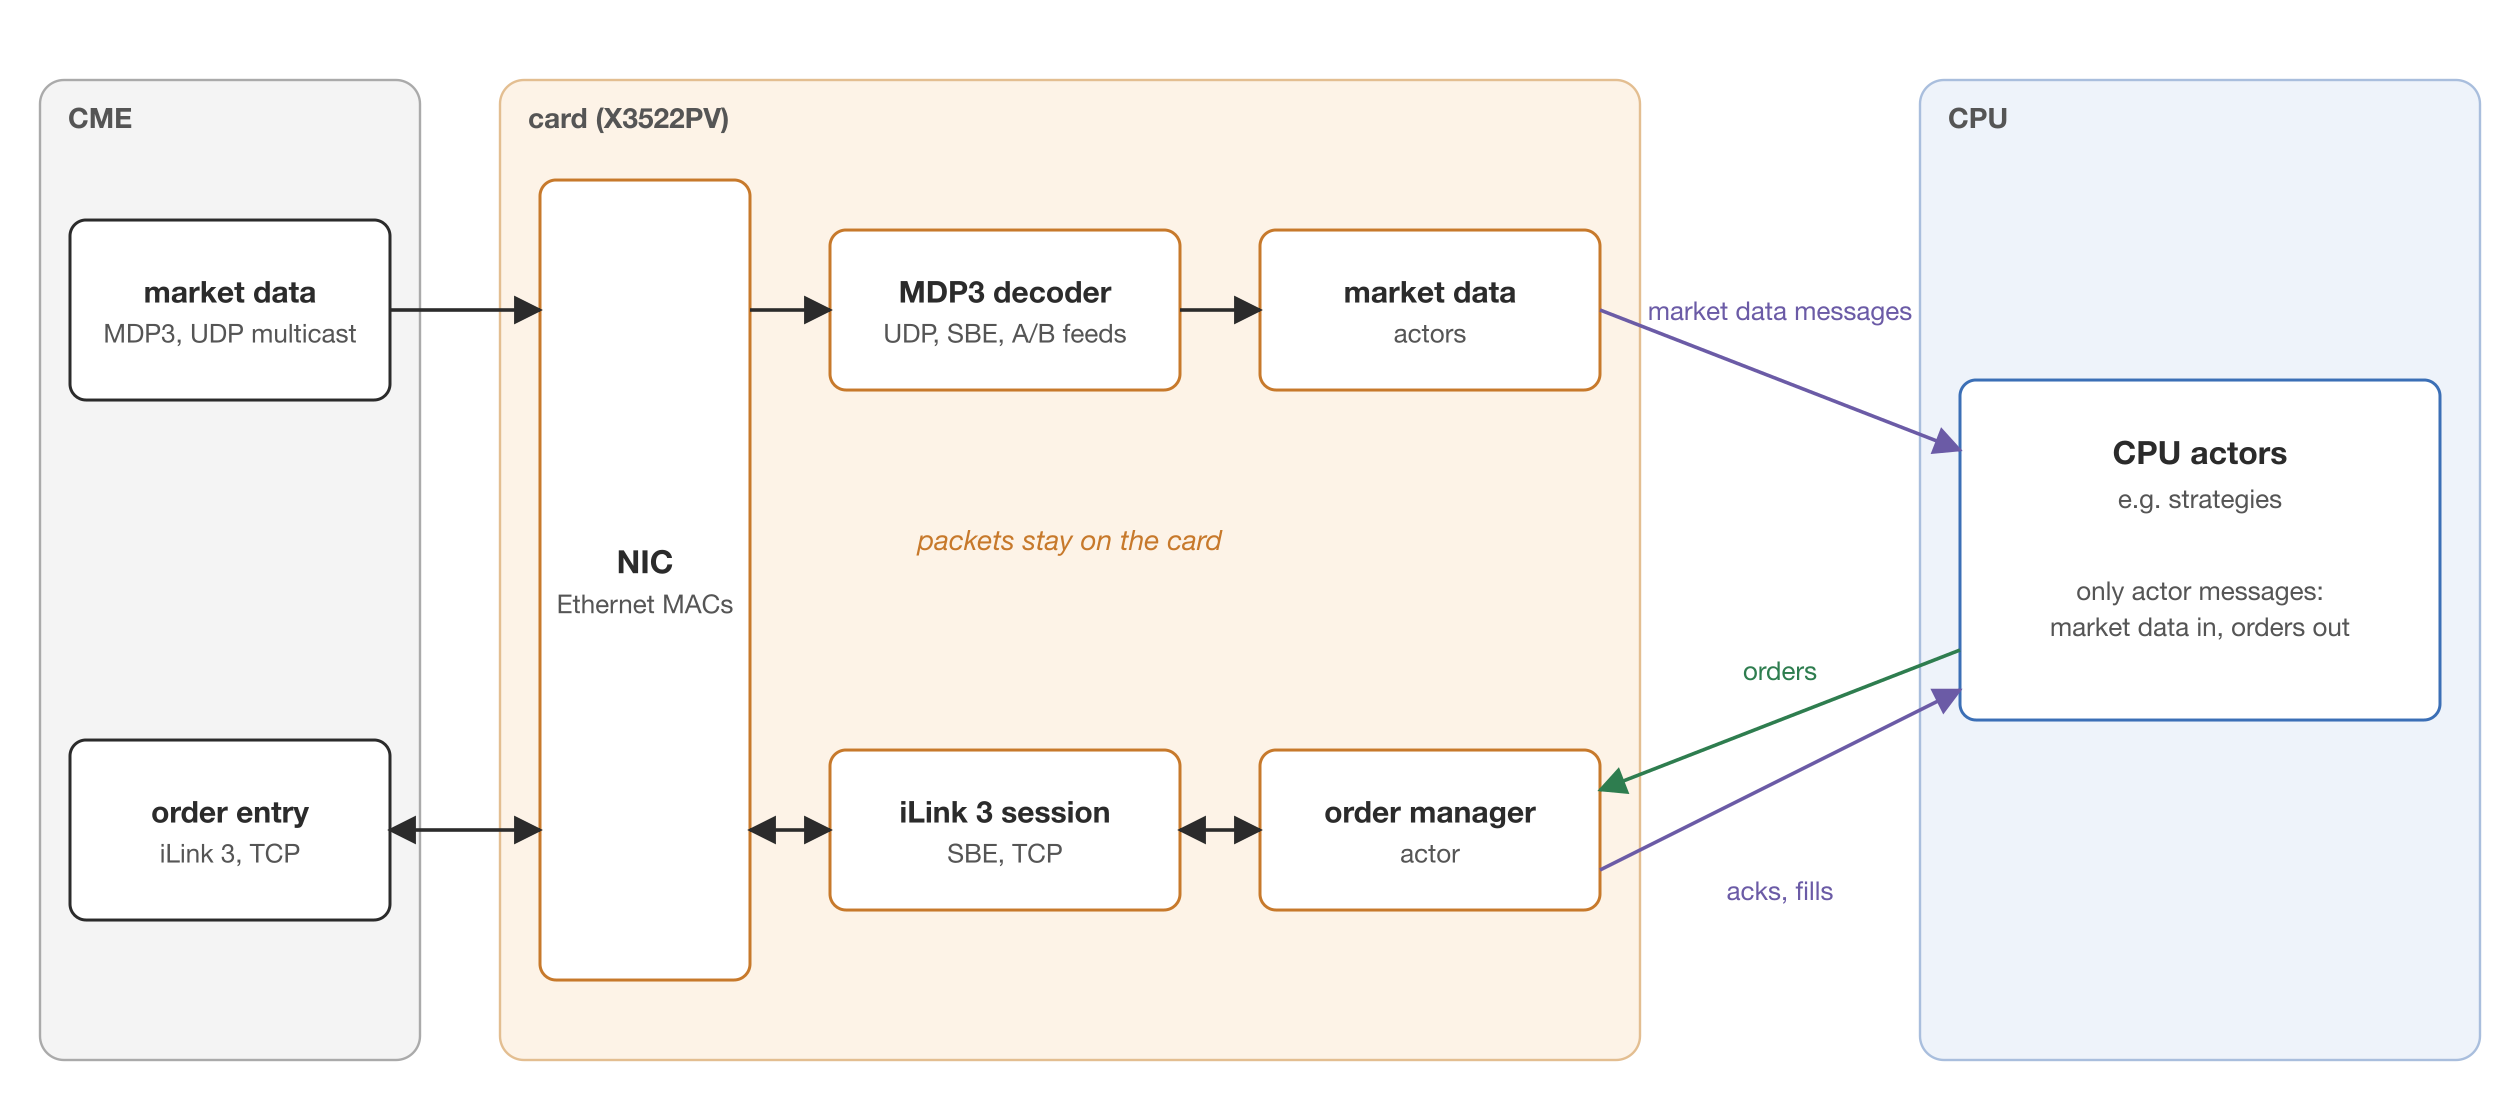
\includegraphics[width=0.95\textwidth]{fig_card_roles.png}
\caption{The card holds the NIC, the MDP3 decoder and iLink~3 order entry. The CPU actors exchange only actor messages with it: market data in, orders out, acknowledgements and fills back.}
\label{fig:cardroles}
\end{figure}

\subsection{Moving data across PCIe}
\label{sec:pcie}

Everything between the card and the CPU travels as PCIe transactions, and for
latency the question that matters is whether a transaction is a write or a read.
A write is \emph{posted}: the sender puts it on the link and carries on. A read
is a round trip: the reader sends a request and waits for the data to come back,
typically 0.5 to 1~$\mu$s, with the reading core stalled the whole time. PCIe also
keeps the writes of one sender in order. The design below follows from these two
facts: each side writes into the other's memory and reads only its own.

\paragraph{Three ways to move data.} The first is \emph{memory-mapped I/O}
(MMIO). The card exposes register windows, its base address registers (BARs),
which the CPU maps into its address space; a store to one of those addresses
becomes a PCIe write to the card. If the window is mapped write-combining, the
CPU gathers up to 64 bytes and normally sends them as one transaction, so a
64-byte message is a single write; this is \emph{programmed I/O} (PIO), the
CPU itself moving the data, and for a small message it is the fastest way onto
the card. A store fence after it makes the CPU send it at once. The second is
\emph{direct memory access} (DMA): the card reads or writes host memory itself.
To send to the CPU, the card writes into a \emph{ring} in host memory, a fixed
array of slots used as a queue (Figure~\ref{fig:ring}), and a CPU thread polls
it. DMA also works the other way, with the CPU writing a descriptor into host
memory and ringing a doorbell, an MMIO write that tells the card where to look;
the card then fetches the data, a read on its side, which suits large or
batched transfers better than single messages. The third is an
\emph{interrupt}: the card sends an MSI-X message, the CPU takes an interrupt and
the driver wakes a sleeping thread, which costs several microseconds plus the
scheduler's jitter. Latency-sensitive receivers poll instead.

\begin{figure}[htbp]
\centering
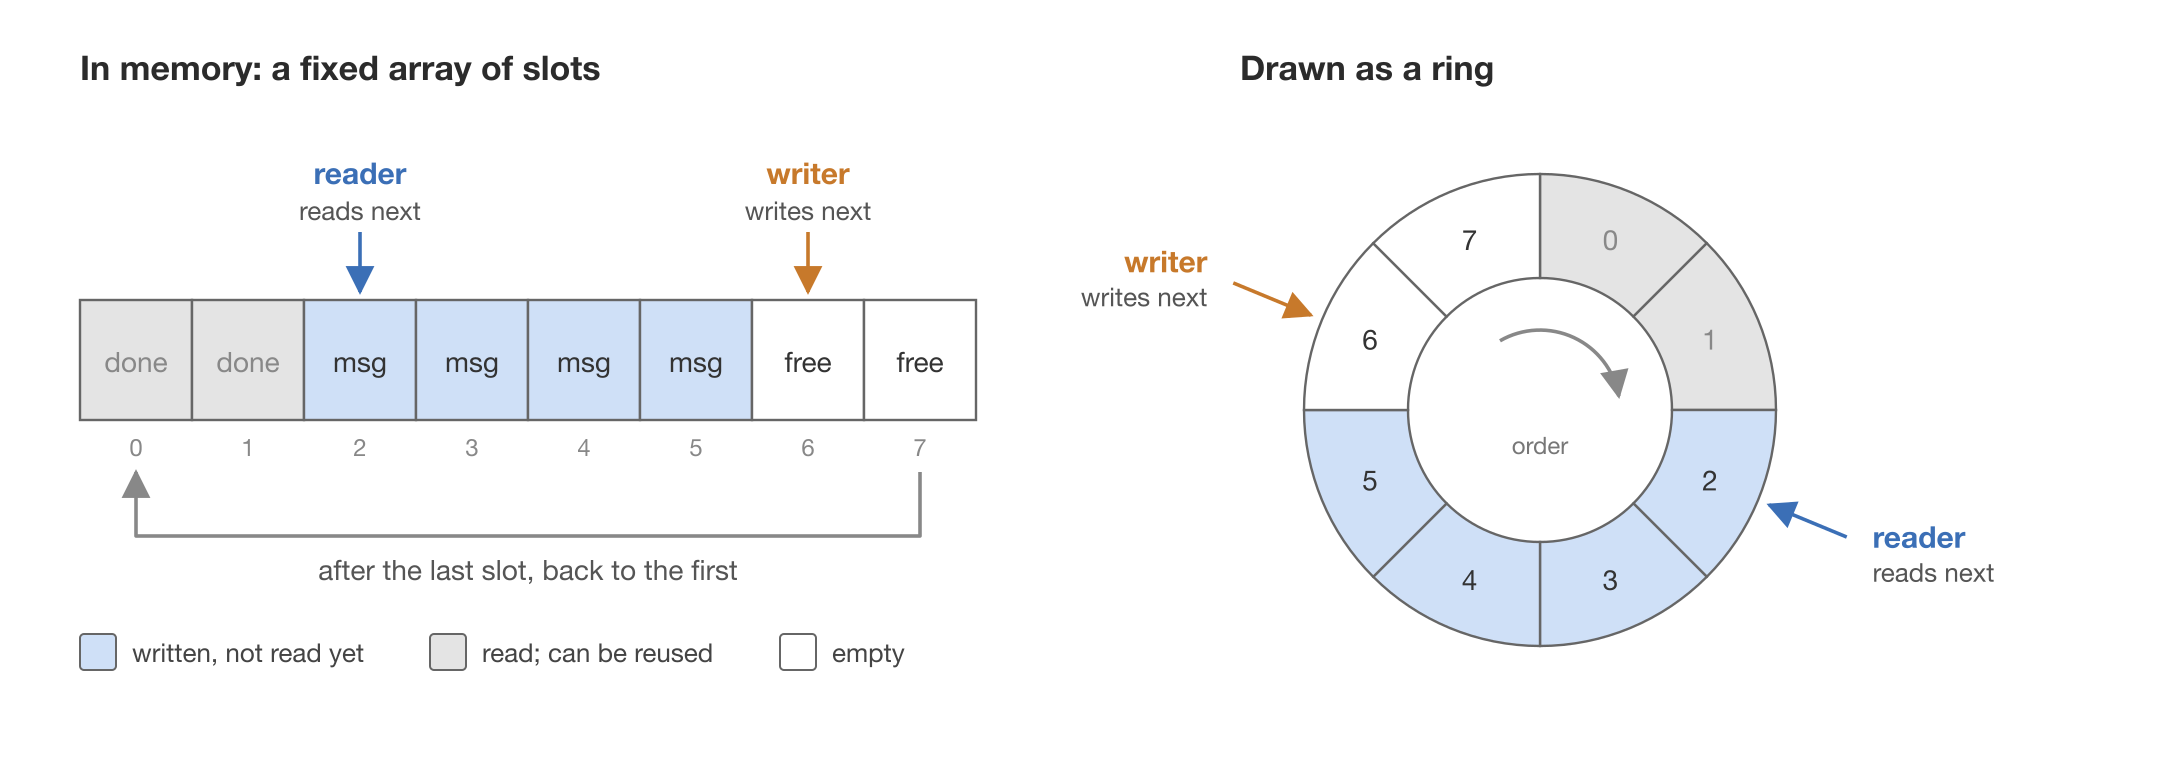
\includegraphics[width=0.85\textwidth]{fig1_ring.png}
\caption{A ring: a fixed array of slots used as a queue. The writer fills the next slot and the reader takes them in the same order; both wrap from the last slot to the first. With one writer and one reader, no lock is needed.}
\label{fig:ring}
\end{figure}

\paragraph{Where a DMA write lands.} If the platform places DMA writes directly
in the CPU's cache (Intel calls this DDIO, Data Direct I/O), the polling thread's
next read hits the cache. If the write goes to main memory instead, it
invalidates the cached line, and the first poll after it costs a trip to memory,
around 100~ns.

\paragraph{Typical costs.} Table~\ref{tab:pciecost} gives typical figures for
PCIe systems in general; they depend on the platform and the PCIe generation and
are not measurements on the X3522PV. An interrupt and wake-up costs more than a
round trip to the card, which is why the receiving side polls; and a synchronous
round trip to the card costs thousands of CPU instructions, which is why a
latency-sensitive loop stays on one side of the link.

\begin{table}[htbp]
\centering
\small
\caption{Typical costs of crossing PCIe (not measured on this card).}
\label{tab:pciecost}
\begin{tabular}{ll}
\toprule
operation & typical cost \\
\midrule
first poll after a DMA write that went to DRAM & $\sim$100~ns \\
PCIe read from the CPU, round trip & 0.5--1~$\mu$s \\
synchronous CPU $\to$ card $\to$ CPU round trip & 1--2~$\mu$s \\
interrupt and thread wake-up & several $\mu$s, plus jitter \\
\bottomrule
\end{tabular}
\end{table}

\paragraph{Staying out of the kernel.} A device normally belongs to a kernel
driver, and a program reaches it through system calls, each of which costs far
more than a memory access. VFIO (Virtual Function I/O), the Linux framework for
handing a device to an ordinary program, removes them from the data path. The
card is bound to the \texttt{vfio-pci} driver, and once, at start-up, the program
makes two mappings: the card's register windows into the program, so a store
through a pointer is a PCIe write to the card; and the program's ring memory to
the card, so the card's DMA engine can write into it. After that, sending is a
store into the card's window and receiving is a load from the program's own
memory, with no system call per message.

The rings are placed in huge pages (2~MB or 1~GB), so a ring needs one address
translation entry rather than one per 4~KB page; the pages are locked in memory,
since the card writes to fixed physical addresses; and the IOMMU, which
translates the card's addresses into real memory addresses, admits the card
only to the memory registered with it (Figure~\ref{fig:ringmem}). A thread that
reads from the card spins on its ring, with a \texttt{pause} instruction on each
empty pass, so it sees each message as soon as it lands.

\begin{figure}[htbp]
\centering
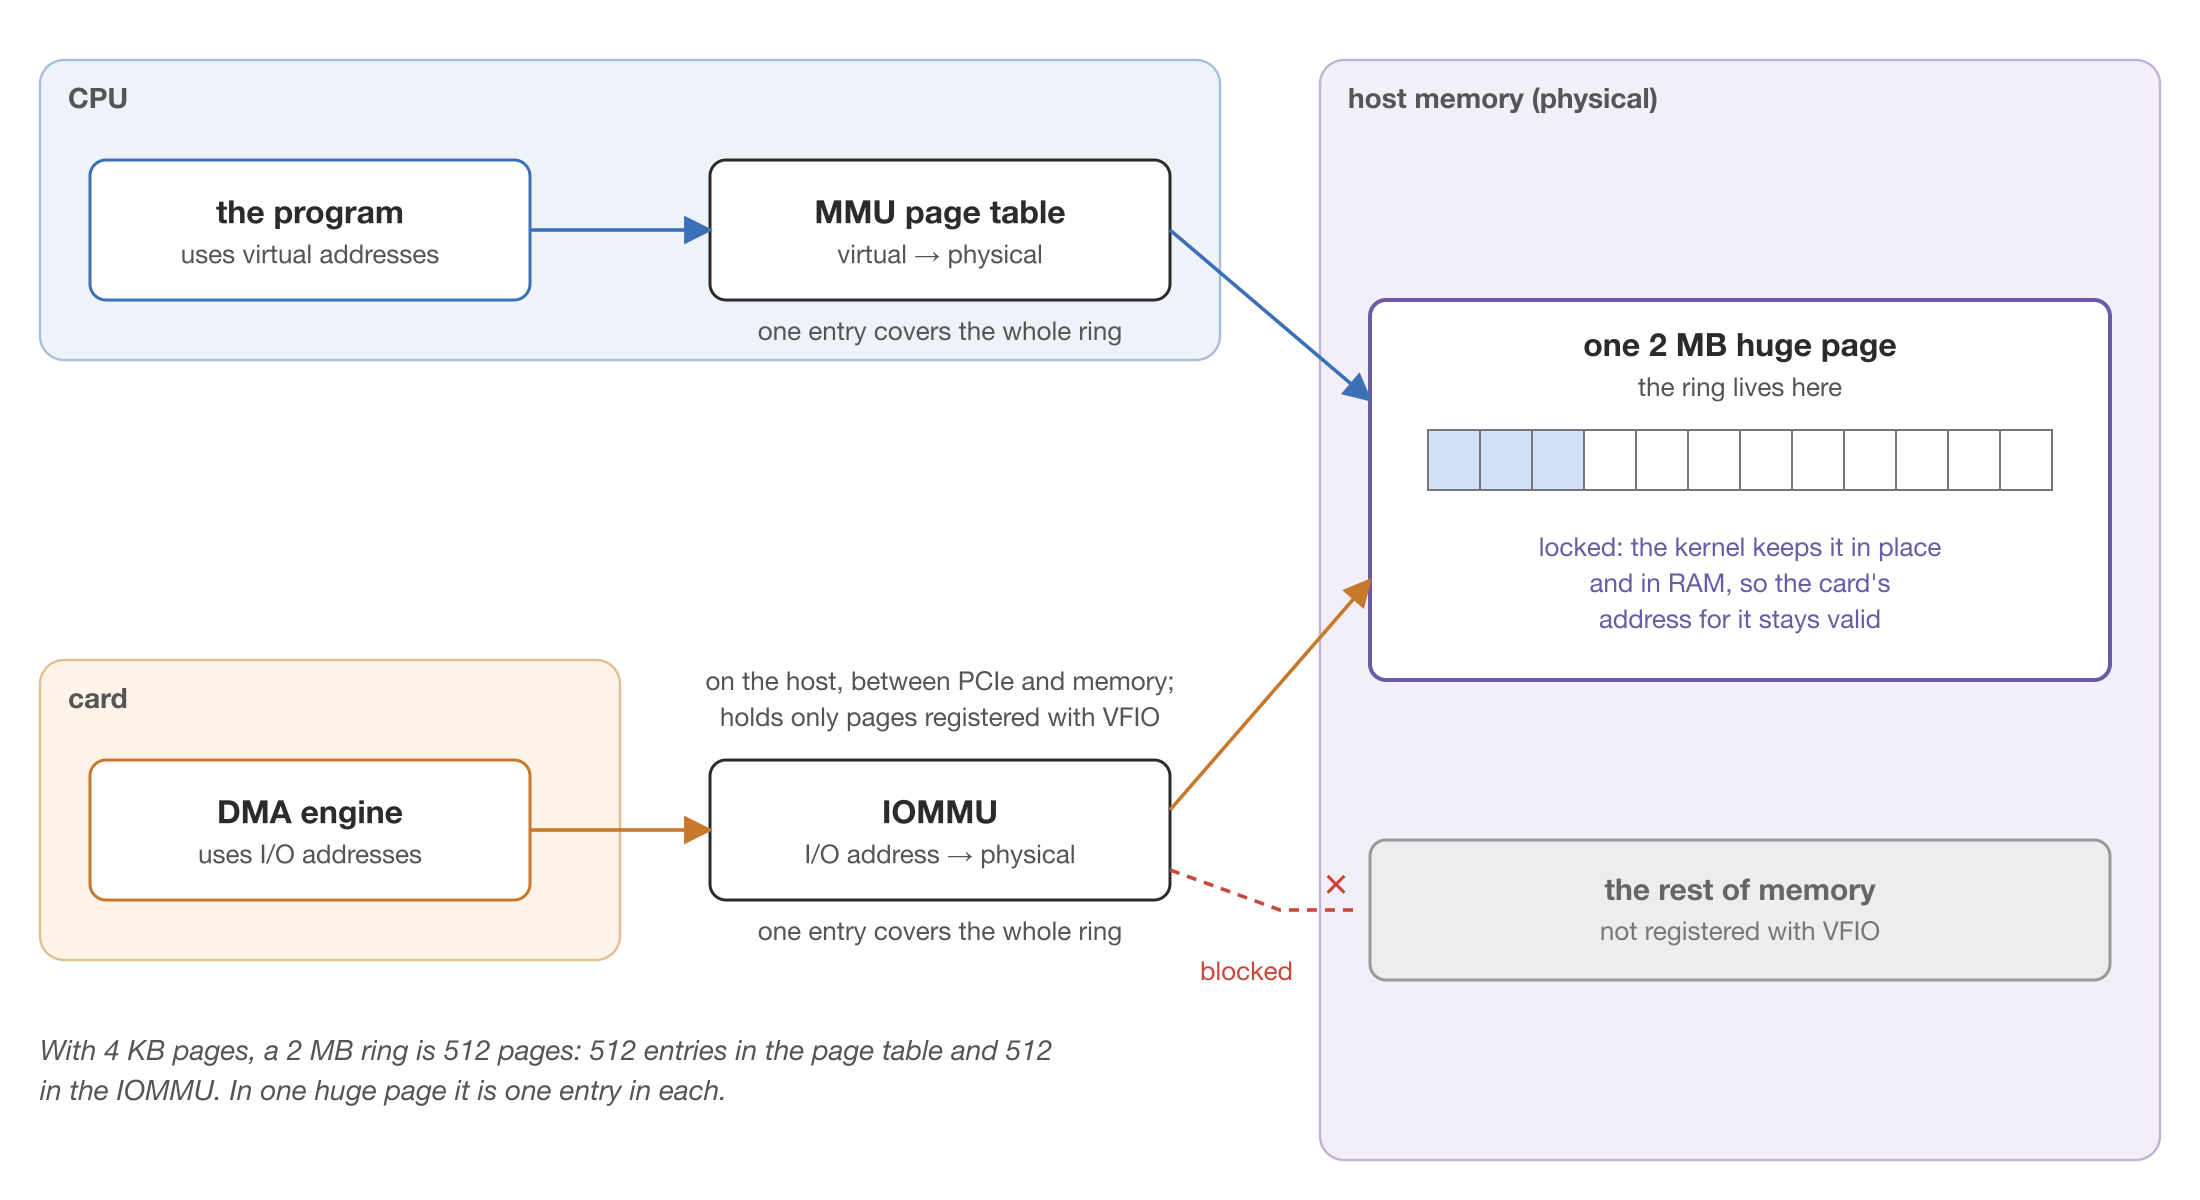
\includegraphics[width=0.9\textwidth]{fig_ring_memory.png}
\caption{The program reaches the ring through the CPU's page table, and the card's DMA engine through the IOMMU. With a huge page each needs one entry for the whole ring; the page is locked, and the IOMMU blocks the card from all other memory.}
\label{fig:ringmem}
\end{figure}


\subsection{The link}
\label{sec:hlink}

The unit of hybrid wiring is a \emph{link}: it joins one CPU actor to one port
of one FPGA process, and consists of two rings, one in each direction, each
with one writer and one reader and slots of one 64-byte envelope. A link has a
\emph{client}, the side that holds a reference to the other and sends first,
and a \emph{server}, which answers with \texttt{reply}. Either side may be the
client. Table~\ref{tab:links} shows the links of the framework's CPU--FPGA
example, in which the same two FPGA actors used on the card alone play against
CPU actors in both directions.

\begin{table}[h]
\centering
\caption{The three links of the CPU--FPGA example. Each FPGA process sees a
link as an ordinary port; each CPU actor sees it as an ordinary actor
reference.}
\label{tab:links}
\small
\begin{tabular}{l l l l}
\toprule
Link & Client & Server & FPGA port \\
\midrule
A & \texttt{CpuPing} (CPU) & \texttt{PongActor} (FPGA) & port 0 of Pong's process \\
B & \texttt{CpuDriver} (CPU) & \texttt{PingActor} (FPGA) & port 0 of Ping's process \\
C & \texttt{PingActor} (FPGA) & \texttt{CpuPong} (CPU) & port 1 of Ping's process \\
\bottomrule
\end{tabular}
\end{table}

\texttt{CpuPing} plays 1{,}000 round trips against \texttt{PongActor} on the
card. \texttt{CpuDriver} sends a start message to \texttt{PingActor} on the
card, which then plays 1{,}000 round trips against \texttt{CpuPong} on the CPU
and reports back to \texttt{CpuDriver}. \texttt{PingActor} and
\texttt{PongActor} are the same source as in the card-only example; only the
design header that plugs their ports in differs:

\begin{lstlisting}
using PingProc = kfpga::Process<PingActor>;
using PongProc = kfpga::Process<PongActor>;

inline void wire()
{
  PingActor &ping = PingProc::member<PingActor>();
  ping.starter = kfpga::ActorRef(0, kCpuDriver);   // port 0: link B, to the CPU
  ping.pong = kfpga::ActorRef(1, kCpuPong);        // port 1: link C, to the CPU
}
\end{lstlisting}

\noindent The CPU actors are ordinary kaspar-hft actors. On the CPU a message is
the class \texttt{kfpga::CpuMsg<P>} built from the same struct; for example,
\texttt{cpu::Ping} is \texttt{kfpga::CpuMsg<pingpong::Ping>}. \texttt{CpuPing} plays
against the FPGA \texttt{PongActor}, and \texttt{CpuPong} answers the FPGA
\texttt{PingActor}; both use the lane mailbox (Section~\ref{sec:lanes}):

\begin{lstlisting}
class CpuPing : public actors::Actor
{
  actors::ActorRef pong_;   // the FPGA PongActor
  uint32_t rounds_;
  uint32_t replies_ = 0;

public:
  explicit CpuPing(uint32_t rounds) : rounds_(rounds)
  {
    set_mailbox(MailboxKind::FpgaLanes);
    MESSAGE_HANDLER(actors::msg::Start, on_start);
    MESSAGE_HANDLER(cpu::Pong, on_pong);
  }
  void set_pong(actors::ActorRef pong) { pong_ = pong; }

private:
  void on_start(const actors::msg::Start *) { pong_.send(new cpu::Ping(1), this); }
  void on_pong(const cpu::Pong *m)
  {
    if (++replies_ < rounds_)
      pong_.send(new cpu::Ping(replies_ + 1), this);
  }
};

class CpuPong : public actors::Actor
{
public:
  uint32_t pings = 0;
  CpuPong()
  {
    set_mailbox(MailboxKind::FpgaLanes);
    MESSAGE_HANDLER(cpu::Ping, on_ping);
  }

private:
  void on_ping(const cpu::Ping *m)
  {
    ++pings;
    reply(new cpu::Pong(m->count));   // back out through the window, on this thread
  }
};
\end{lstlisting}

\noindent (\texttt{CpuPing} is shown without the reporting code of the example
program.) The CPU actors' code is that of any kaspar-hft actor: they \snd{} to
an \texttt{ActorRef} and \texttt{reply}, and do not know that their peer is on
the card.

\subsection{Naming the other side}
\label{sec:naming}

\paragraph{From the CPU.} A CPU actor holds an ordinary kaspar-hft actor
reference to the FPGA actor. The reference points to a \emph{stand-in}: a CPU
object of the actor class that represents the FPGA actor on the CPU and never
runs a thread of its own. Its \snd{} encodes the message into an envelope,
stamps the source and destination actor ids of the link, and writes it into
the link's outbound ring, on the thread of the CPU actor that called it. The
CPU actor's handlers are those of any CPU actor, and its \snd{} is the usual
call.

\paragraph{From the card.} An FPGA actor holds an ordinary FPGA actor
reference: a port number and the destination's actor id
(Section~\ref{sec:nopointers}). The port is plugged into the card's PCIe side
instead of another process's FIFO, and the actor id is the CPU actor's. The
FPGA actor's handler sends exactly as it would to a peer on the card.

\paragraph{Replies.} A message arriving on the CPU from the card is delivered
with the stand-in as its sender, so the CPU actor's \texttt{reply} goes to the
stand-in and back out through the link. A message arriving on the card from
the CPU comes in on the link's port, so the FPGA actor's \texttt{reply} goes
out on that port and back across the bus. Neither side needs to know that the
other is not local.

\subsection{One message, two forms}
\label{sec:twoforms}

A message type is declared once, as a struct with a hand-assigned id and a list
of integer fields (Section~\ref{sec:envelope}), in a header compiled into both
programs. On the card it is used as it is. On the CPU a template,
\texttt{CpuMsg<F>}, makes it an ordinary kaspar-hft message with the same
fields and the same id, so a CPU actor registers a handler for it as for any
other message, and constructs one with \texttt{new} as usual.

Between the two forms stands a \emph{codec}: a table, indexed by message id,
of two functions per message type that may cross the link. One encodes a CPU
message's fields into an envelope's payload; the other decodes an envelope onto
the stack of the receiving thread and runs the target's handler on it. Each
side of the system lists the message types that cross its links, once, and a
message with no entry is counted as an error rather than delivered. No message
is allocated on the receiving side: the decoded message lives on the stack for
the duration of the handler, as a \fs{} request does in the CPU framework.

\subsection{The transport: windows and lanes}
\label{sec:transport}

Each ring of a link is placed so that its writer writes across the bus and
its reader reads its own memory (Figure~\ref{fig:link}), because a PCIe write
is posted and a PCIe read is a round trip (Section~\ref{sec:requirements}).

\begin{figure}[h]
\centering
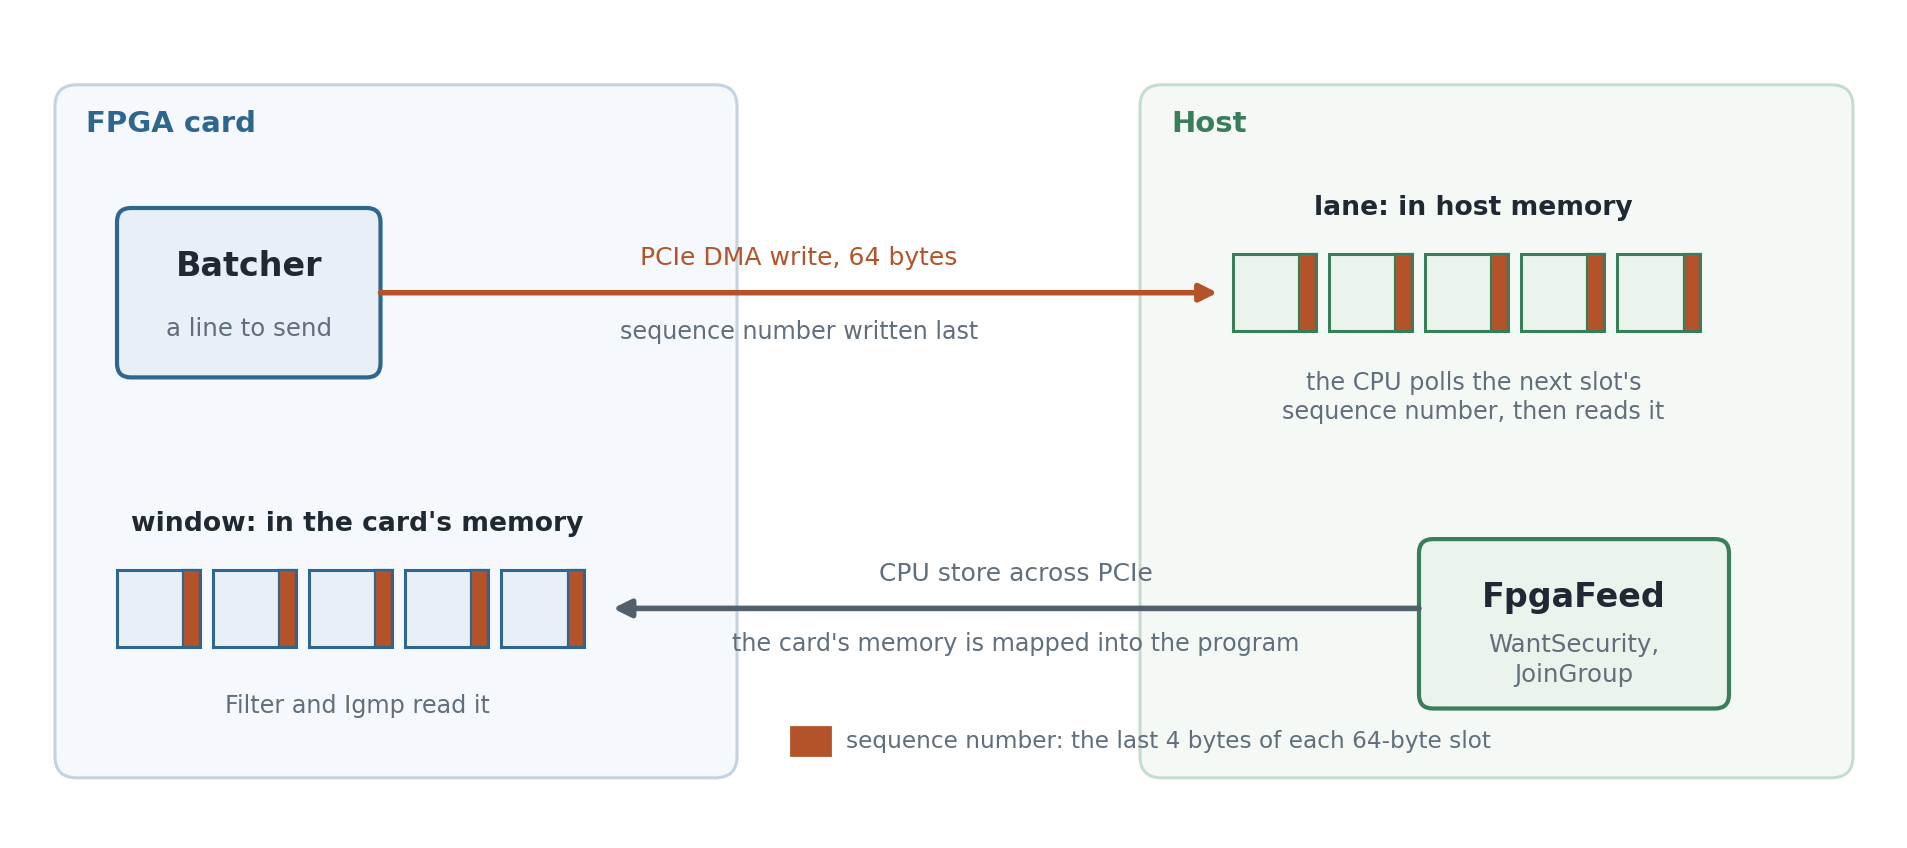
\includegraphics[width=0.92\textwidth]{pcie_link.png}
\caption{The two rings of a CPU--FPGA link, shown for the market-data handler
of Section~\ref{sec:casestudy}. The card writes 64-byte slots into a lane in
host memory by DMA, the sequence number last; the CPU writes into a window in
the card's memory with ordinary stores. Each side reads only its own memory.}
\label{fig:link}
\end{figure}

\paragraph{Card to CPU: the lane.} The lane is a ring in host memory, owned by
the thread that will handle its messages. The card writes each envelope into
the next slot with a PCIe DMA write; the thread watches the sequence number of
the next slot in its own cache, and when it changes, the slot is complete.

\paragraph{CPU to card: the window.} The window is a ring in the card's memory,
exposed through a PCIe base address register and mapped into the program, so
the CPU thread writes a slot with ordinary stores --- on hardware, one
write-combined 64-byte burst and a fence --- which reach the card as posted
writes. The card reads the window in its own memory.

Each CPU actor that talks to the card has its own window and its own lane
(Figure~\ref{fig:lanes}), so every ring has exactly one writer and needs no
lock.

\begin{figure}[htbp]
\centering
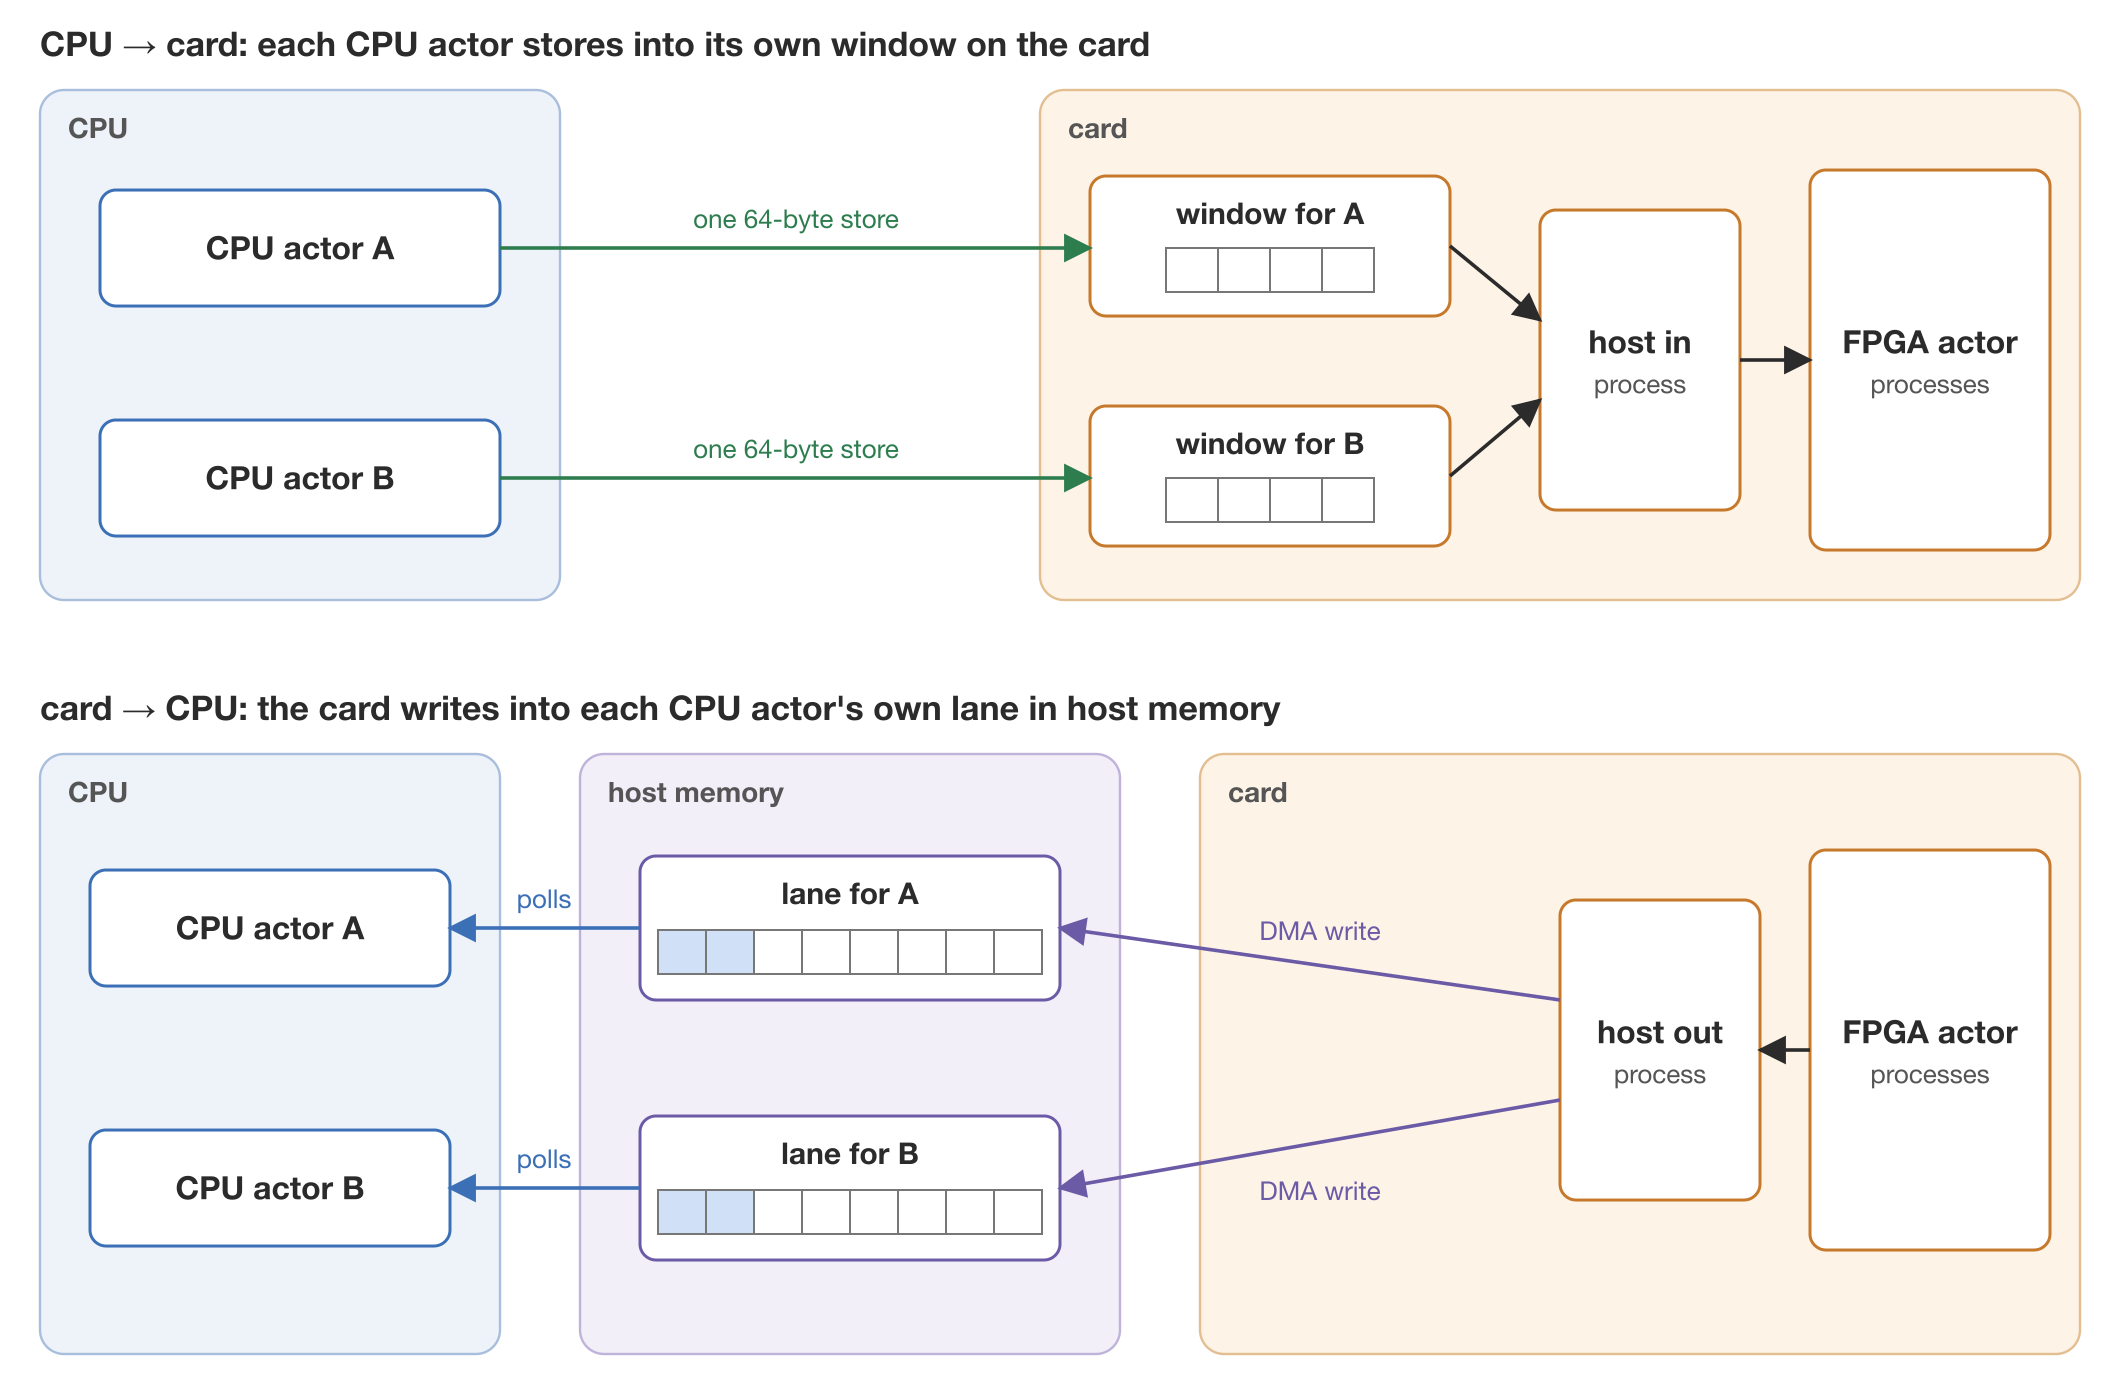
\includegraphics[width=0.92\textwidth]{fig4_lanes.png}
\caption{Each CPU actor stores into its own window on the card, and the card writes into each CPU actor's own lane in host memory.}
\label{fig:lanes}
\end{figure}

\paragraph{Sequence number last.} A slot is one 64-byte cache line: the 60-byte
envelope followed by a 32-bit sequence number (Figure~\ref{fig:slot}), so one
message is one write going to the card and one cache line coming back. The
writer copies the envelope's 60 bytes of header and payload, then stores its
4-byte sequence number with release ordering; the reader loads the sequence number with acquire ordering and takes
the slot once it sees the number it expects. The 64-byte copy need not be
atomic: only the aligned 4-byte sequence number is waited on, and the writer
guarantees it lands last. On the card side this relies on PCIe delivering posted
writes in order, which holds with relaxed ordering disabled for the DMA
engine's writes, and on the engine writing the sequence number after the rest
of the slot. There are no locks and no atomic read-modify-write operations on
the path.

\begin{figure}[htbp]
\centering
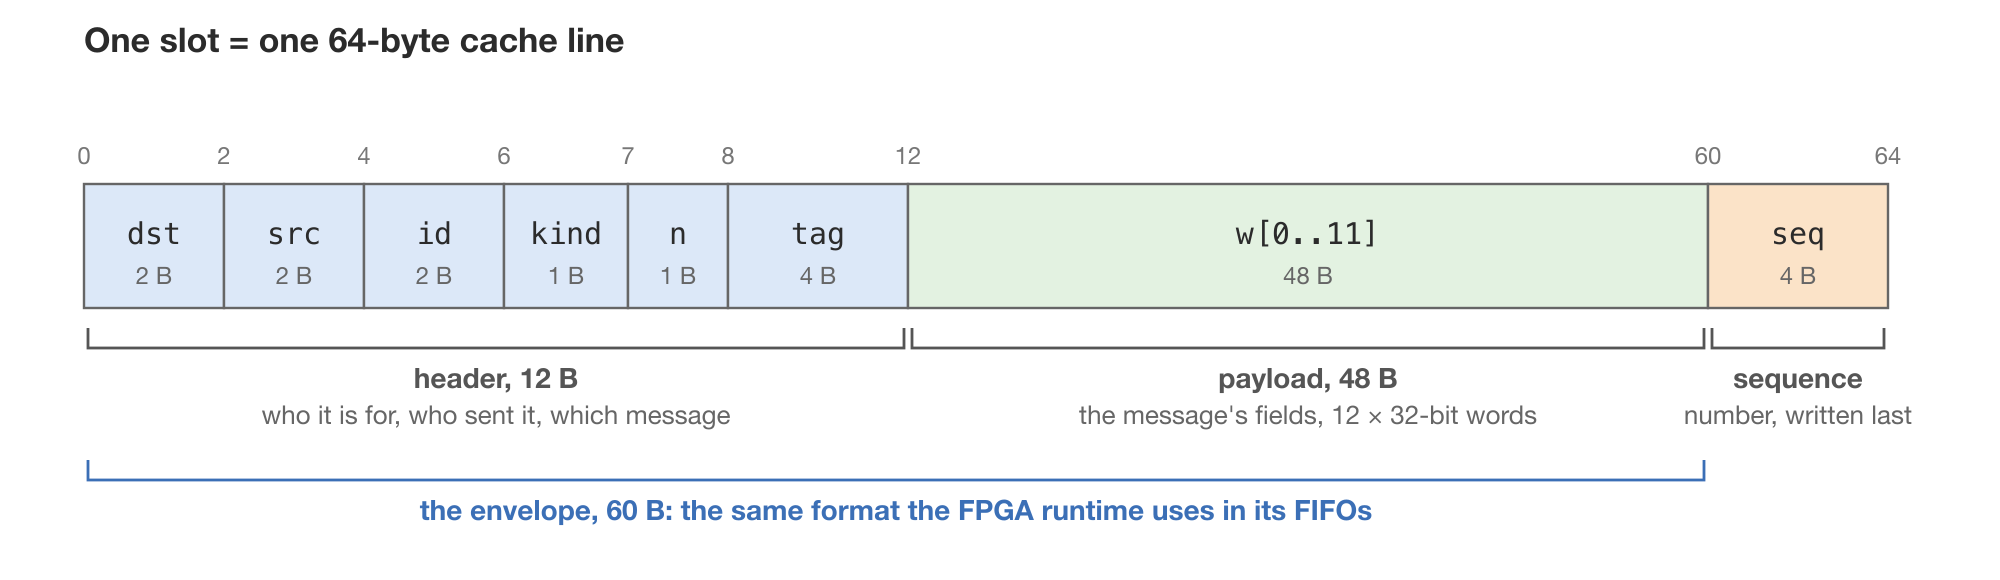
\includegraphics[width=0.95\textwidth]{fig2_slot.png}
\caption{One slot is one 64-byte cache line: a 60-byte envelope, in the same format the FPGA runtime uses in its FIFOs, followed by a 32-bit sequence number written last.}
\label{fig:slot}
\end{figure}

\paragraph{Batched positions.} A writer must know when a ring is full, which
requires the reader's position. The reader publishes its position every quarter
of the ring, or when it finds the ring empty; the writer keeps a copy and
refreshes it only when the ring appears full. Position updates therefore cross
the bus a few times per ring rather than once per message.

\paragraph{The card's side.} One DMA engine serves every link. Inbound, each
link's window is its own address range, so the engine knows from where an
envelope was written which link, and hence which process port, it belongs to.
Outbound, the envelope's destination actor id names the lane, and the engine
writes it there. In the HLS designs the engine is modelled by one stream in
each direction and two small dataflow functions that distribute the inbound
envelopes to the links' ports and collect the outbound ones; on a card, the DMA
engine takes their place. The CPU side of the transport is built and tested
against a software card; the DMA engine is designed but not yet built.

\subsection{A message's path, end to end}
\label{sec:path}

One round trip of link~A, \texttt{CpuPing} to \texttt{PongActor} and back,
takes the following path.

\begin{enumerate}[leftmargin=1.6em]
  \item \texttt{CpuPing}'s handler calls \snd{} on its reference to
  \texttt{PongActor}, with a \texttt{Ping} created as any CPU message is.
  The call reaches the stand-in, which, on \texttt{CpuPing}'s thread, encodes
  the message into an envelope on the stack, frees the message, and writes the
  envelope into link~A's window: one 64-byte write across the bus.
  \item On the card, the DMA side takes the envelope from link~A's window and
  writes it into the FIFO of port~0 of \texttt{PongActor}'s process.
  \item \texttt{PongActor}'s process takes it on its next step, runs
  \texttt{on\_ping}, and the handler's \texttt{reply} places a \texttt{Pong}
  in the outbox for port~0. The process writes it to port~0's outbound FIFO
  in the same step.
  \item The DMA side writes the envelope into the lane of its destination,
  \texttt{CpuPing}: one DMA write into host memory, sequence number last.
  \item \texttt{CpuPing}'s thread, polling its mailbox, sees the sequence
  number change, decodes the \texttt{Pong} onto its stack, and runs
  \texttt{on\_pong} with the stand-in as sender.
\end{enumerate}

\noindent No thread other than \texttt{CpuPing}'s is involved on the CPU,
nothing reads across the bus, and nothing is allocated on the receiving side. Each direction costs
one posted write across PCIe and a step of the card's process; the reverse
direction, link~C, is the same with the roles exchanged.

\subsection{No routing thread: the lane mailbox}
\label{sec:lanes}

A natural design would have one host thread own the card: it would poll every
lane and forward each message to its recipient's mailbox. That thread is a hop.
In the companion paper's study, the path that handed each datagram to a second
thread through a mailbox had a socket-to-book median of about $7~\mu$s against
about $1~\mu$s on one thread, and part of its tail was mailbox backlog; the runs
also differed in load and configuration, so not all of the difference is the
hop \cite{fastsend}. There is no such thread here (Figure~\ref{fig:bridge}
shows the design that was rejected). Every crossing is written by the thread
that has the message and read by the thread that will handle it.

\begin{figure}[htbp]
\centering
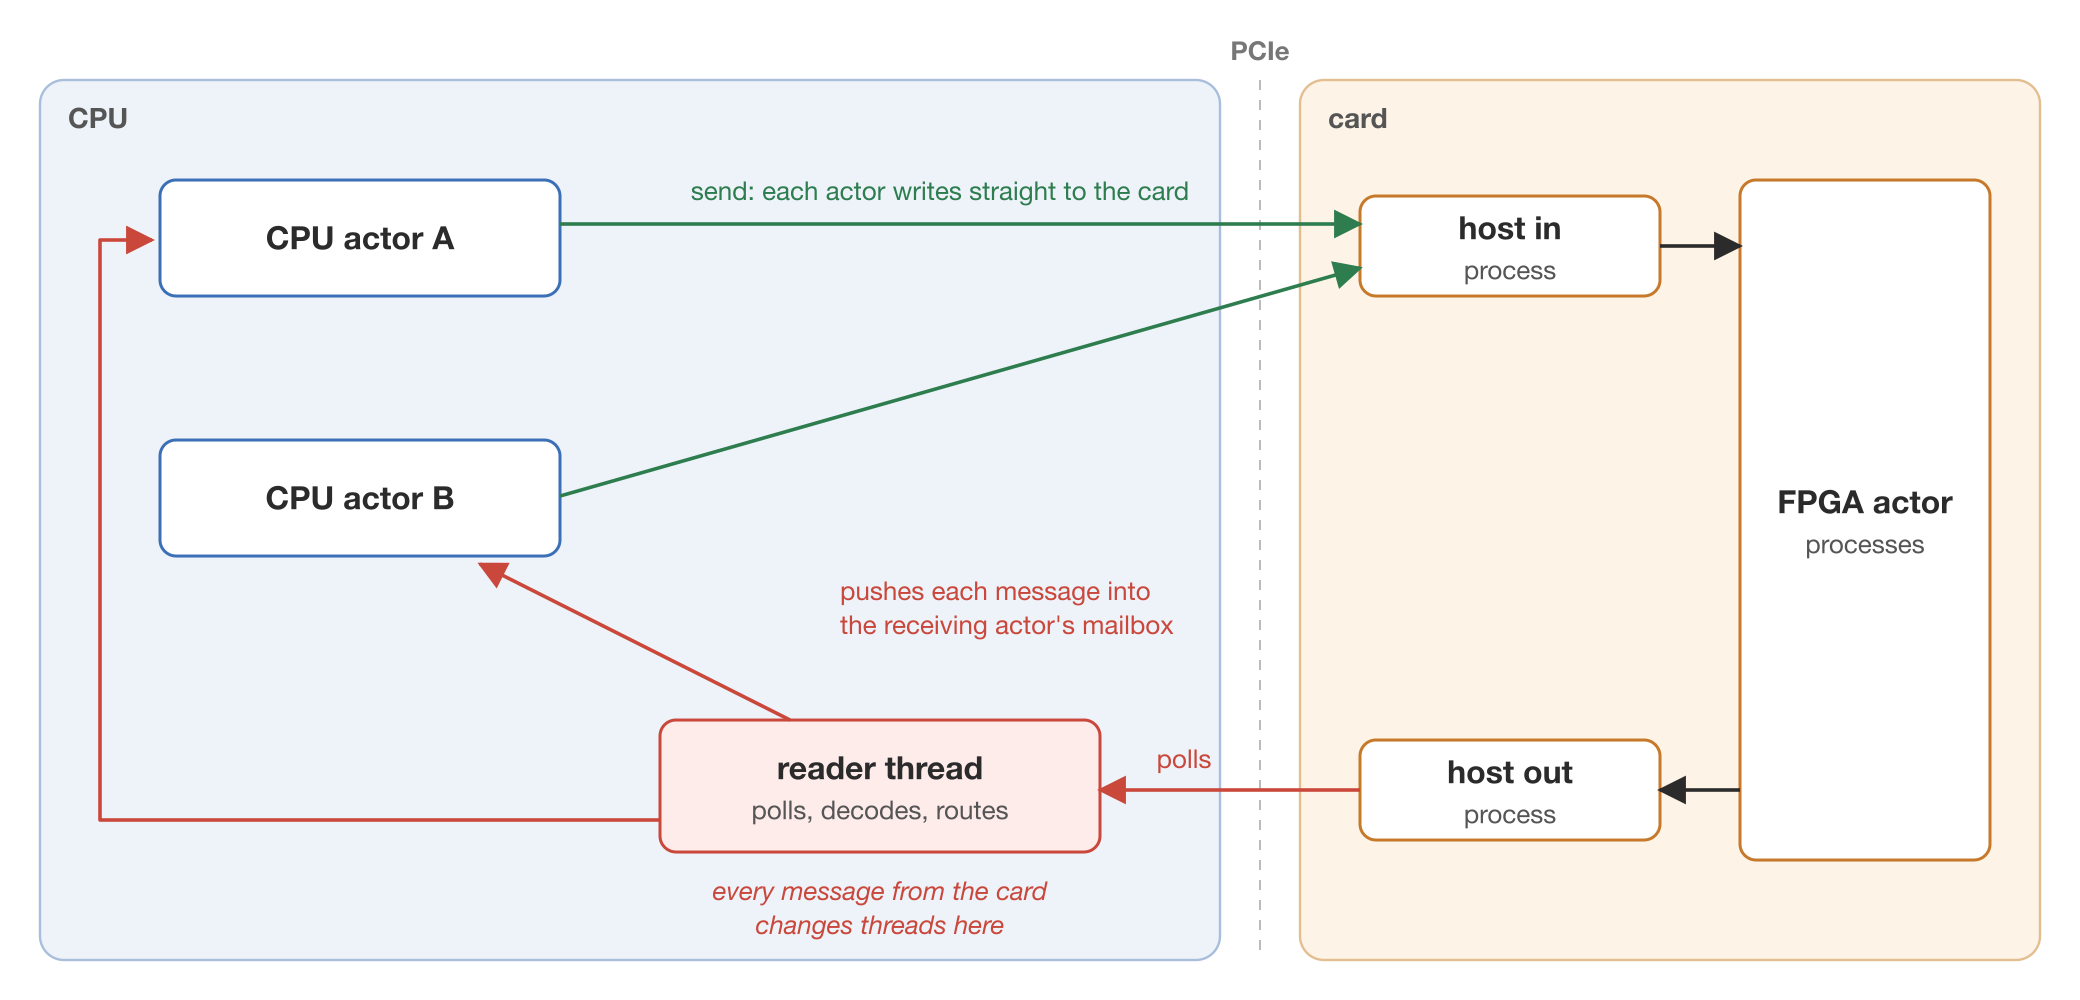
\includegraphics[width=0.9\textwidth]{fig3_first_bridge.png}
\caption{The rejected design: CPU actors write straight to the card, but everything from the card goes through one reader thread that polls, decodes and routes, so every message from the card changes threads.}
\label{fig:bridge}
\end{figure}

On the CPU side this required a new mailbox kind in the actor framework,
\texttt{FpgaLanes}. It is the framework's lock-free multi-producer queue, which
CPU actors push into as before, plus a list of lanes. Its owner's loop checks
each lane and then the CPU queue, one message from each per pass, so a CPU
actor receives from CPU peers and from the card through one mailbox, in one
loop, on one thread (Figure~\ref{fig:fpgalanes}). The loop never sleeps: a thread can sleep on a condition
variable, which CPU senders signal, or on an interrupt, which the card raises,
but not on both, so it spins and checks both. Actors that receive from the card
are put in one group, so they share one spinning thread.

A lane belongs to the thread that polls the mailbox. A member of a group runs
on the group's thread, so its lanes are moved to the group's mailbox, whether
the actor joins the group before or after its lanes are added. An actor that is
given a lane without a lane mailbox stops the program with a message in every
build, since otherwise no thread would ever read the card's messages.

\begin{figure}[htbp]
\centering
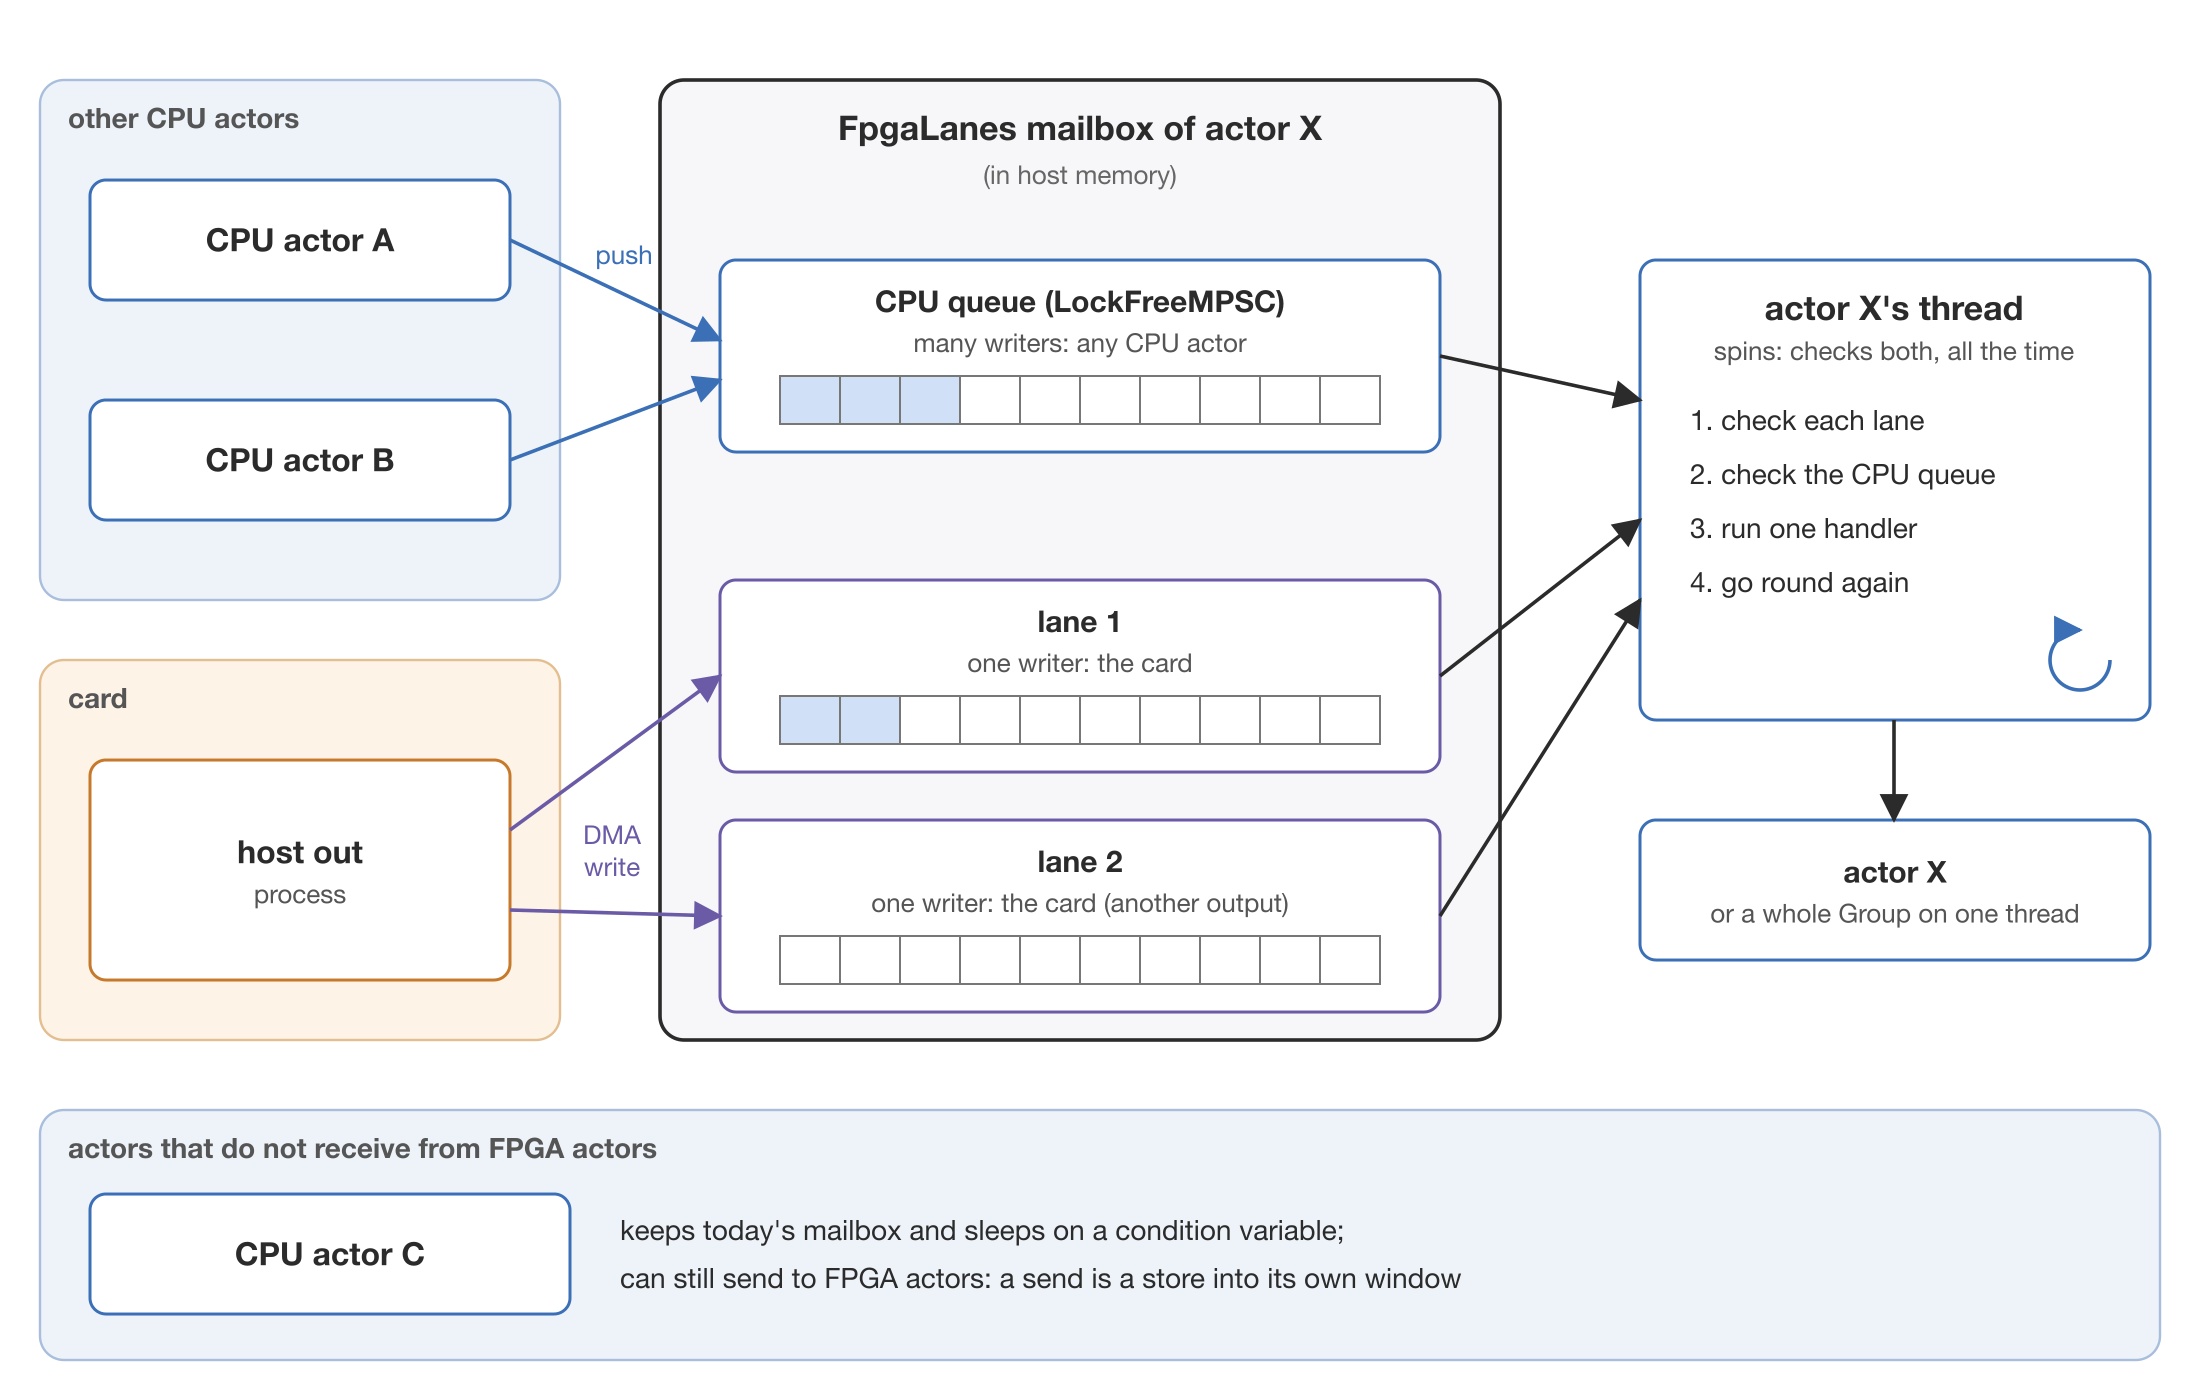
\includegraphics[width=0.92\textwidth]{fig5_fpgalanes.png}
\caption{The FpgaLanes mailbox. CPU actors push into its CPU queue, the card writes into its lanes, and only the owning thread reads both, spinning. Actors that do not receive from the card keep an ordinary mailbox and can still send to it.}
\label{fig:fpgalanes}
\end{figure}

\subsection{Receiver transparency across the link}
\label{sec:transparency}

The companion paper defined receiver transparency as the property that a
handler executes the same code, and does not depend on, whether it was invoked
synchronously or asynchronously, on which thread, or whether its sender is
blocked \cite{fastsend}. Across the link the property extends to location. In
the CPU--FPGA example, \texttt{CpuPong} answers \texttt{PingActor} with the same
handler it would use for a CPU peer, and \texttt{PingActor} plays
\texttt{CpuPong} with the same handler it uses against \texttt{PongActor} on the
card. Moving an actor across the boundary changes the wiring --- the design header,
the link set-up, the receiving CPU actor's mailbox kind and the codec's list of
messages --- not the actor's handlers or its peers'. As in the companion
paper, this is a property of the interface, not one the language enforces.

\subsection{No blocking across the link}
\label{sec:noblock}

A CPU send to the card never waits for the card. If the window is full, the
envelope waits in the CPU end of the link, in order, and the mailbox's poll
loop sends it on as room appears. A blocking send would deadlock: the thread
that sends into the window is the same thread that drains the lane, so a send
blocked on a full window while the card's answers fill the lane leaves both
sides waiting on each other. A test sends far more messages in one handler than
the link holds, to an FPGA actor that answers each, and passes only if every
answer arrives.

Sends to the card can come from more than one thread, because a CPU actor's
handlers can run on the thread of a caller's \fs{} and its reference can be
passed on. They are serialized in the CPU end of the link by a short spin lock,
uncontended when one thread sends, so the window keeps one writer at a time; a
second test sends from several threads at once and checks that every envelope
arrives whole, once, and in each thread's order.

\fs{} is not offered across the link. It would be a \snd{} followed by a
blocking wait for the reply, a round trip across PCIe with the caller's thread
stalled, which is the cost \fs{} exists to avoid. Across the link a request and
its reply are two messages, as between processes on the card. An order from a
CPU strategy to the order manager on the card is one store into the strategy's
window, after which the strategy goes on handling other messages; the
acknowledgement comes back later, written into the strategy's lane, and is
handled when its next poll finds it (Figure~\ref{fig:reqreply}).

\begin{figure}[htbp]
\centering
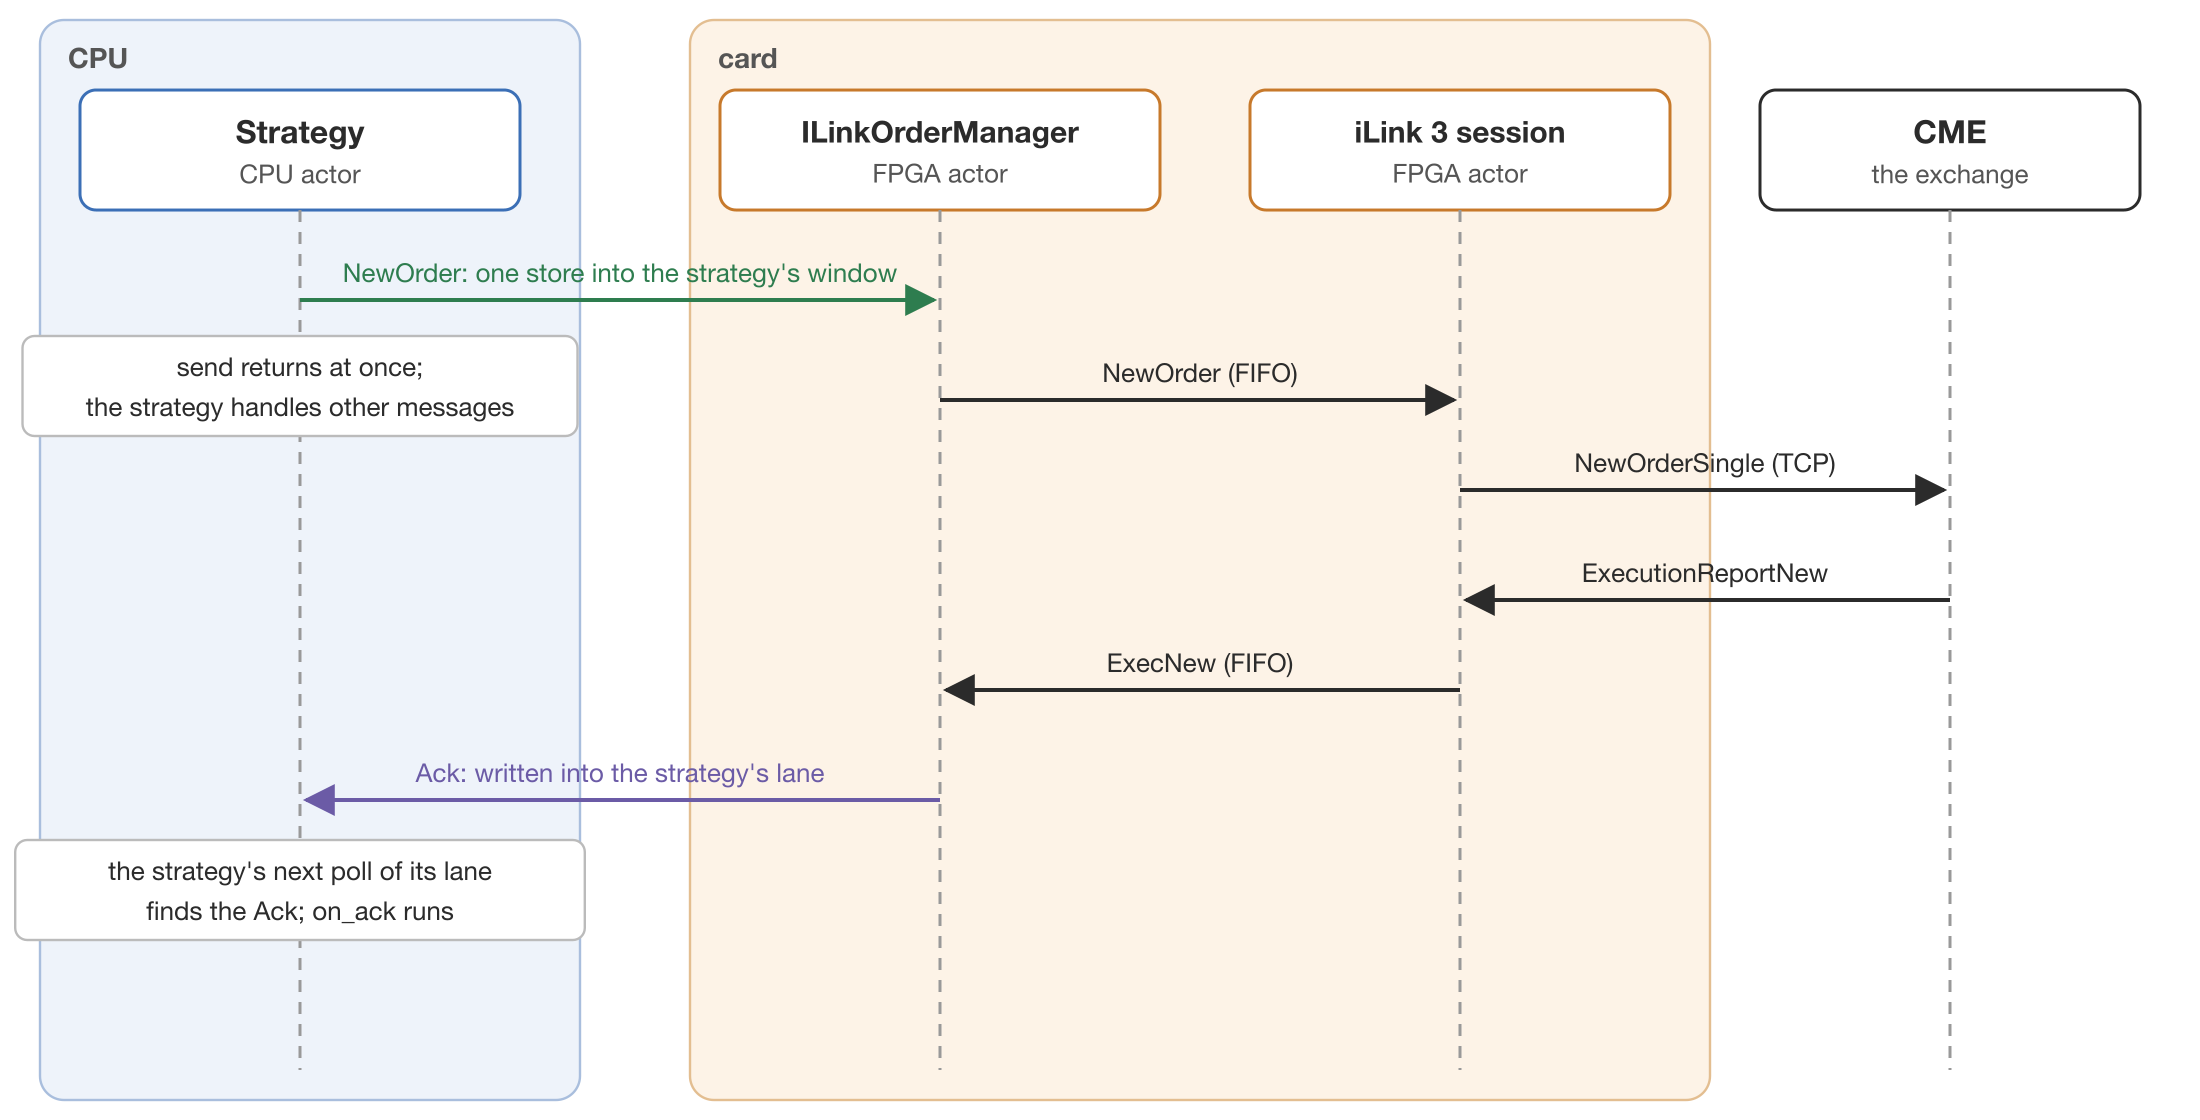
\includegraphics[width=0.95\textwidth]{fig6_request_reply.png}
\caption{An order and its acknowledgement across the link are two messages. The strategy's send returns at once; the acknowledgement arrives in its lane and is handled on a later poll.}
\label{fig:reqreply}
\end{figure}

\subsection{Where to put the boundary}
\label{sec:boundary}

Each crossing costs a posted write across the bus, several hundred nanoseconds
from the card to host memory (Section~\ref{sec:budget}), against a few cycles
between processes on the card and tens of nanoseconds for a \fs{} on the CPU
\cite{fastsend}. The boundary therefore belongs where the traffic is least and
where nothing waits on a reply. In the market-data handler of
Section~\ref{sec:casestudy}, it falls after Filter and Batcher: every byte of the
feed is handled on the card, and only the events of the securities the strategy
trades cross, three to a line. The control traffic, from the CPU to the card,
is a few messages at start. A boundary placed earlier, before the decoder,
would carry the whole feed across the bus and leave the decode on the CPU; one
placed later, after the books, would leave the strategy reading them across the
bus. The cost model is the same as the companion paper's for placing actors on
threads: a hop is cheap within a process and expensive across one, so a
pipeline is cut where little crosses.

\subsection{Testing a hybrid system}
\label{sec:hybridtest}

The two halves of a hybrid design are tested separately, and both with the same
actor source. In software, the CPU actors run on their own threads, as in
production, against a software card that runs the FPGA processes, either
stepped or one thread each, with software rings for windows and lanes; this is
the only configuration in which the CPU side reacts to the card, and it
exercises the codec, the stand-in, the lane mailbox and the no-blocking rule. In
Vitis HLS, the card's half is synthesized and co-simulated against a testbench
that stands in for the CPU actors, envelope by envelope, through the one
stream each way that models the DMA engine. The CPU--FPGA example passes both;
in RTL co-simulation, 2{,}001 envelopes in and 2{,}001 out take 2{,}008 cycles,
one message a cycle in both directions at once (Section~\ref{sec:perf}). The
PCIe transport itself --- windows, lanes and the DMA engine on a real card --- is
not yet tested.

% ---------------------------------------------------------------
\section{From software to hardware: verification}
\label{sec:verify}
% ---------------------------------------------------------------

A design is three small files: a design header that declares the processes
and their wiring, shared by the software run and the HLS top so that the two
cannot drift apart; an HLS top with one task per process and two streams per
link; and a testbench. It is checked at four levels.

\begin{enumerate}[leftmargin=1.6em]
  \item \textbf{Plain C++.} The framework compiles without HLS, with a
  software ring in place of each FIFO. A software card runs the processes either
  stepped, deterministically, or on a thread each, against real CPU actors. This
  checks the actors' logic and the CPU side of the link, and nothing about
  timing or resources.
  \item \textbf{C simulation.} The design is compiled the way HLS compiles it
  and run against the testbench.
  \item \textbf{Synthesis.} The design becomes RTL, and the report gives each
  process's latency, its II, the estimated clock and the resources.
  \item \textbf{RTL co-simulation.} The generated Verilog is simulated, cycle
  by cycle, with the same testbench, and its outputs are compared with C
  simulation.
\end{enumerate}

Each of the rules below was found because a design passed C simulation and
failed a later level (Table~\ref{tab:rules}). Several concern the boundary of a
free-running design: a design made only of tasks returns as soon as it starts,
and polls its inputs with non-blocking reads that co-simulation cannot drive on
a top-level port. The tops therefore include a small counted boundary --- plain
dataflow functions that move a known number of envelopes between the top-level
ports and the tasks --- so that the top returns when its work is done. On a
card, the boundary is the DMA engine and the MAC, and the counting functions do
not exist.

\begin{table}[h]
\centering
\caption{Rules forced on the framework by synthesis and co-simulation.}
\label{tab:rules}
\small
\begin{tabular}{p{4.6cm} p{4.4cm} p{4.4cm}}
\toprule
Symptom & Cause & Rule \\
\midrule
synthesis: pointer to pointer not supported & a pointer stored in an object and followed later & no stored pointers (Section~\ref{sec:nopointers}) \\
co-simulation: a flood of all-zero envelopes & a stream kept inside an actor object of a task; HLS builds no FIFO & every FIFO is declared at the top level and plugged in \\
synthesis: a stream with no producer & a one-actor process with a group queue nothing writes & an own queue only for two or more members \\
co-simulation hangs & non-blocking reads on a top-level port of a free-running design & actors poll only internal streams; the boundary uses blocking reads \\
co-simulation scrambles the order on a link & a top of tasks only returns at once & the counted boundary \\
co-simulation hangs after a speed-up & uninitialized envelopes are unknown (X) in RTL & every envelope starts at zero, by an unrolled loop \\
II~$=2$ on a process & one FIFO read from two places & read each port from exactly one place \\
synthesis does not finish & pipelining unrolled a 1{,}024-round handler loop & pipeline only processes whose handlers have no long loops \\
synthesis removes an actor's output & HLS treats the actor's object as constant & handlers run through the group's step \\
\bottomrule
\end{tabular}
\end{table}

The last row is not understood. Three actors were affected: HLS decided that an
actor's single object never changes, read every member as its initial value,
and removed the actor's output with everything that depended on its state,
reporting the problem far from its cause. Running the actor's handlers through
the group's ordinary step cured it in every case, and an actor that both reads
and writes raw streams is held directly in its task. We have no explanation of
why HLS does this, or of why an actor of the same kind, the decoder, was never
affected.

% ---------------------------------------------------------------
\section{Performance of the framework on the card}
\label{sec:perf}
% ---------------------------------------------------------------

The examples in \texttt{actors/fpga} play 1{,}000 round trips between two
actors in three configurations: two processes on the card, three actors in one
group, and the card's half of a CPU--FPGA exchange with the testbench standing
in for the CPU. They were synthesized for a Kintex UltraScale+ KU5P at 250~MHz,
a device of the same generation as the target card's, covered by AMD's free
license, and run in RTL co-simulation (Table~\ref{tab:perf}).

\begin{table}[h]
\centering
\caption{The framework on the card: RTL co-simulation on the KU5P at
250~MHz. Before and after the changes of Section~\ref{sec:pipeline}.}
\label{tab:perf}
\small
\begin{tabular}{p{6.6cm} r r}
\toprule
& First version & Pipelined \\
\midrule
One step, the replying actor & 33--64 cycles & 1 cycle \\
One step, the initiating actor & 33--59 cycles & 2 cycles \\
Initiation interval & 33+ cycles & 1 cycle \\
Actor-to-actor round trip on the card & 92 cycles, $\approx$370~ns & 5 cycles, 20~ns \\
CPU--FPGA example: 2{,}001 envelopes in, 2{,}001 out & 56{,}996 cycles & 2{,}008 cycles \\
Group: 1{,}000 \snd{} + 1{,}000 \fs{} round trips & 139{,}124 cycles & 32{,}033 cycles \\
Two-process example, size & 4{,}885 FF, 7{,}793 LUT & 1{,}785 FF, 1{,}462 LUT \\
\bottomrule
\end{tabular}
\end{table}

The CPU--FPGA example moves one message a cycle in both directions at once.
The group example is left unpipelined because one of its handlers loops
(Section~\ref{sec:pipeline}), so a \snd{} round trip through the group's own
queue still costs about 30 cycles, while a \fs{} costs about 2 cycles a call.
Synthesis estimated the clock at about 342--344~MHz for all three designs, each
of which uses about 1\% of the KU5P.

These figures do not include PCIe. A round trip between a CPU actor and an FPGA
actor is dominated by the bus, which costs several hundred nanoseconds each way
(Section~\ref{sec:budget}); the framework's own cost on the card is a few
cycles.

% ---------------------------------------------------------------
\section{Case study I: the CME MDP3 handler on the Alveo X3522PV}
\label{sec:casestudy}
% ---------------------------------------------------------------

\subsection{The tail of a software handler}

CME publishes market data as UDP multicast packets in MDP3, encoded in Simple
Binary Encoding (SBE) \cite{fixsbe,cmemdp3}. A packet carries a sequence number
and one or more messages; a book-update message carries a repeating group of
entries, one per changed price level, and the exchange coalesces the events
available at each send into one packet. When the market moves, packets are long
and arrive back to back.

A software handler, with or without kernel bypass, takes a packet once the NIC
has delivered all of it, then decodes its messages in sequence. Its time after
the packet's last byte grows with the packet; and when long packets arrive back
to back, each waits for the decode of the one before. The companion paper's
socket-to-book measurements on live CME futures show the consequence: on one
thread, book-update medians of $0.8$--$1.1~\mu$s, but 99.9th percentiles of
$8.8$ to $69.3~\mu$s for book updates and up to $124~\mu$s for trades, related
there to the clustered arrival process \cite{fastsend,mdarrival}.

On a card whose network port is wired to the FPGA, the packet can instead be
decoded as it arrives. If every stage takes one step per clock and keeps up
with the wire, then by the time a packet's last byte arrives every entry before
it has been decoded, and only a fixed number of clocks of work remain, for a
long packet as for a short one.

\subsection{The design split}

The target is an AMD Alveo X3522PV \cite{ug1523}, a network card whose 10/25~GbE
ports are wired to an XCUX35 FPGA. The handler is split between the card and the
host (Figure~\ref{fig:system}). The card does all the work that grows with the
packet: the Ethernet, IP and UDP headers, the SBE decode, dropping the
instruments the strategy does not trade, and packing what remains into 64-byte
lines. It also subscribes to the multicast group itself. The CPU builds the
order books from the lines and runs the strategy. The card keeps no book: one
book per instrument means many books, and the strategy, which runs on the CPU,
would read them across PCIe in any case. A book on the card pays only once the
trading decision is on the card too.

\begin{figure}[h]
\centering
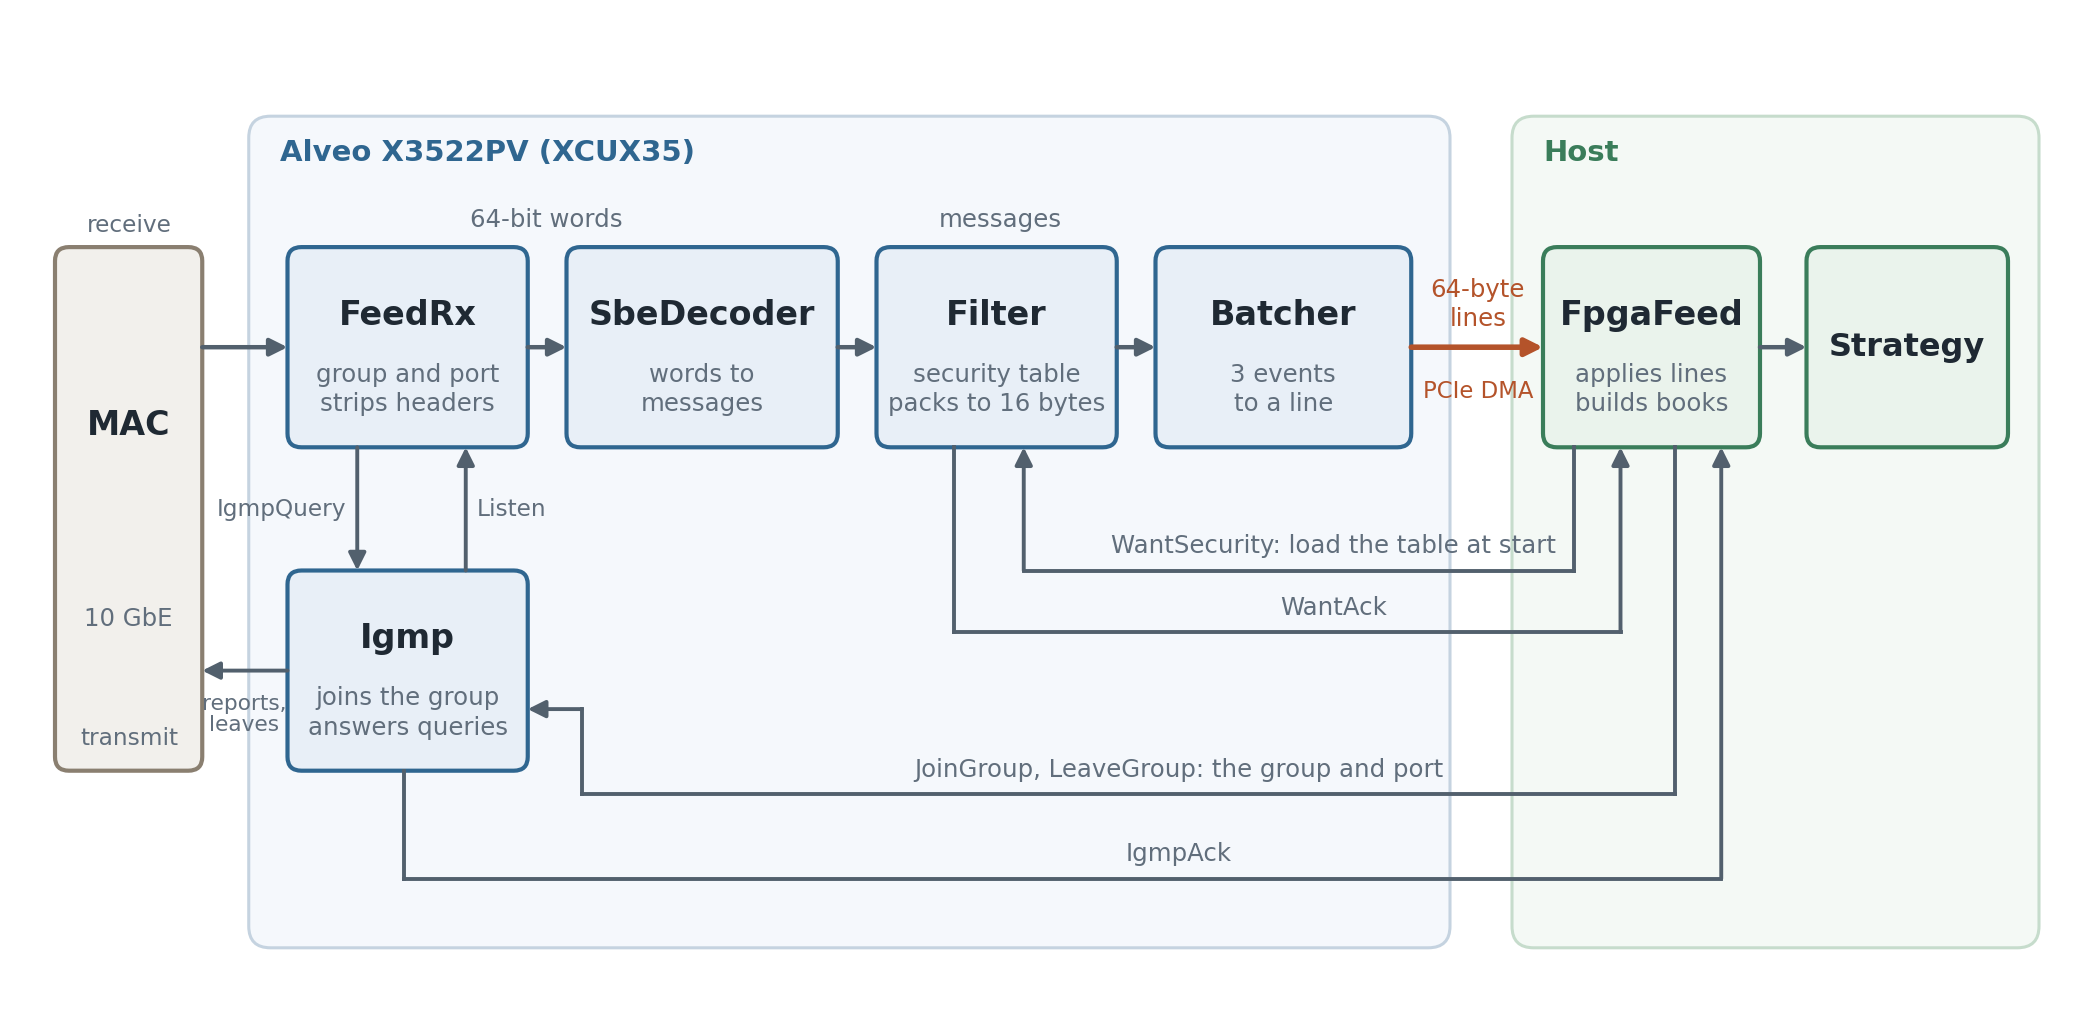
\includegraphics[width=\textwidth]{system.png}
\caption{The MDP3 handler: five actors on the card, one on the CPU. FeedRx and
SbeDecoder take 64-bit words; the others take messages. Lines cross to the host
by DMA; the host loads Filter's table and asks Igmp to join the group, through
the window.}
\label{fig:system}
\end{figure}

Every stage, on the card and on the CPU, is an actor
(Table~\ref{tab:actors}). Each actor on the card is a process of its own and
takes one step per clock.

\begin{table}[h]
\centering
\caption{The actors of the handler.}
\label{tab:actors}
\small
\begin{tabular}{p{2.0cm} p{1.0cm} p{4.2cm} p{5.6cm}}
\toprule
Actor & Where & Input & Output \\
\midrule
FeedRx & card & Ethernet frames, 64-bit words & the UDP payloads of one group and port, realigned to word boundaries \\
Igmp & card & the host's join and leave; the switch's queries, from FeedRx & IGMPv2 reports and leaves to the MAC; the group to FeedRx \\
SbeDecoder & card & payload words & one message per wanted entry; an end-of-packet with the sequence number \\
Filter & card & decoded messages; the security table, from the host & 16-byte packed events of wanted securities \\
Batcher & card & packed events & 64-byte lines of three events; one End line per packet \\
FpgaFeed & CPU & lines, from the lane & the books, to the strategy \\
\bottomrule
\end{tabular}
\end{table}

\subsection{The actors}

\paragraph{FeedRx} receives frames from the MAC as 64-bit words. Every header of
a frame lies in its first six words, so when the sixth arrives FeedRx checks
every field it needs at once --- IPv4, UDP, the configured group and port ---
in one clock, with comparators wired to fixed positions. It strips the 42 bytes
of Ethernet, IP and UDP header (46 with a VLAN tag), and realigns the payload,
which begins 2 bytes into a word, by joining the tail of each input word to the
head of the next: one word in and one out every clock, at a cost of one word of
delay. The UDP length gives the end of the payload, so Ethernet padding never
reaches the decoder. The group and port are not known when the design is built;
Igmp supplies them in a message when the host joins. FeedRx sends no messages
on its main path, only raw words, and runs on the raw-stream step.

\paragraph{Igmp} joins the multicast group. A switch forwards a multicast group
only to ports that have asked for it with an IGMP membership report. On an
ordinary NIC the kernel sends that report; here the port belongs to the FPGA,
so an actor on the card does. At the host's request, Igmp tells FeedRx the group
to accept and sends a 60-byte IGMPv2 report \cite{rfc2236}, repeated once; it
answers the switch's periodic queries, which FeedRx passes to it, and sends a
leave when the host leaves. It writes its frames to the MAC without waiting, so
FeedRx is never held up by it.

\paragraph{SbeDecoder} takes payload words and stores nothing beyond a two-word
window and a 32-byte register. From the window it can take 8 bytes starting at
any byte offset, so a message or field that straddles two words costs no
throughput. It never handles a message as a whole: every clock it takes the next
8 bytes, or fewer at the end of a part, and a state machine
(Figure~\ref{fig:decoder}) decides what they are from three counters loaded from
the wire --- bytes left in the message, entries left in the group, bytes left in
the entry. Length is counted, not processed. When an entry's 32 bytes are in the
register, decoders generated from CME's XML template read its fields at fixed
offsets and the entry goes to Filter as a message. Book updates, trades,
security status and channel resets are read; every other template, and the
order-level group of book updates, is skipped by its size counter, 8 bytes a
clock. The decision of how many bytes a step consumes sets where the next step
reads, and is the design's timing-critical path; it is taken from the state and
from flags precomputed into registers rather than from comparisons in the step.

\begin{figure}[h]
\centering
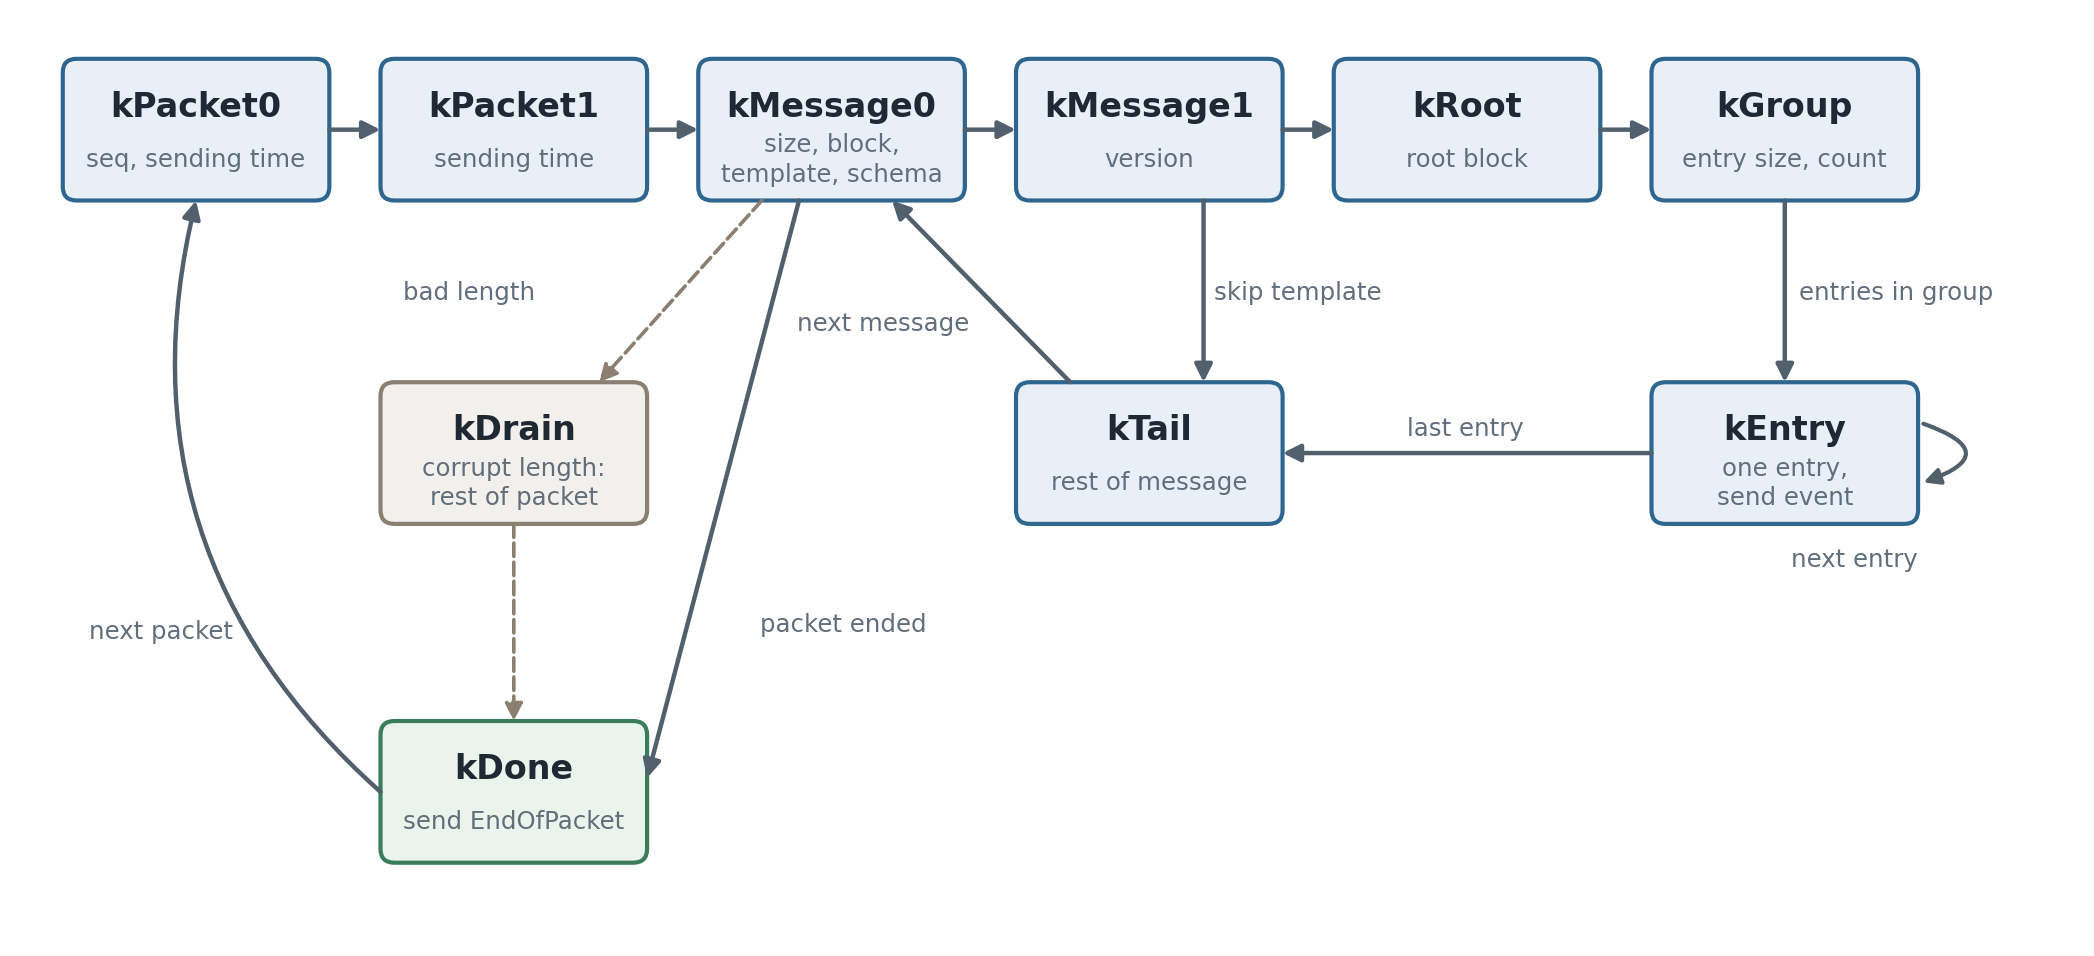
\includegraphics[width=0.78\textwidth]{decoder_states.png}
\caption{The states of SbeDecoder. Each step consumes up to 8 bytes; the
counters loaded from the message size, the group header and the entry size
choose the next state.}
\label{fig:decoder}
\end{figure}

A 32-byte entry takes the decoder 4 clocks, 16~ns at 250~MHz; the same 32
bytes take 25.6~ns to arrive at 10~Gb/s. However many entries a group holds,
each is decoded before the next has arrived.

\paragraph{Filter} keeps the securities the strategy trades. The host loads a
table of up to 64 security ids at start, one message per entry, each
acknowledged; an entry's security id is compared with all 64 at once, in one
clock, however full the table. Filter drops implied entries, which are most of
the traffic on some channels, and every security outside the table, and packs
each surviving entry into a 16-byte event in which the security's position in
the table replaces its 4-byte id, so the host indexes its array of books
directly. Security status, channel resets and every end-of-packet always pass.

\paragraph{Batcher} puts three events in each 64-byte line and sends a line as
soon as its third event arrives, while the rest of the packet is still on the
wire. At the end of each packet it sends an End line carrying the sequence
number and the 0--2 events left over; every packet produces exactly one End
line, so the host sees every sequence number and can detect a gap even in a
packet with nothing for it. Nothing waits for a timer or for the next packet,
and there is one send per step, so Batcher runs at II~$=1$.

\paragraph{FpgaFeed} is an ordinary kaspar-hft actor on a lane mailbox. At
start it loads Filter's table and asks Igmp to join, and reports ready when
every entry and the join are acknowledged. It applies each full line to its
books the moment it lands, while the rest of its packet is still arriving, so
when a packet's End line arrives at most two events remain. It checks the
sequence number, sets a gap flag that stays set if a packet was skipped, and
hands the books to the strategy. Because full lines are applied before their
packet's sequence number is known, a late duplicate packet would already have
changed the books; FpgaFeed sets the gap flag in that case too. The handler
reads one feed and does not recover lost packets.

\subsection{Results}
\label{sec:results}

\paragraph{Correctness.} The decoder was checked against the C++ codec that
kaspar-hft's software handler uses, over one full session of CME channel~344
(Treasury futures), feed A: the two produced the same 331{,}183{,}779
decoded records, with none different. RTL co-simulation of the four receive
actors on the card's device, on 2{,}000 consecutive packets of the session,
produced output identical to the C++ model. The design with Igmp added has been
synthesized and placed and routed, and its tests pass in C++ and C simulation,
but it has not yet been co-simulated.

\paragraph{The work after the last byte.} The same actor code compiles as
plain C++, with each process's step called once per simulated clock. All
30{,}044{,}560 packets of the session were run through this model, fed at
10~GbE line rate, with six securities in the table. From a packet's last byte
into FeedRx to its End line out of Batcher took a mean of 5.2 clocks and a
maximum of 8, and the maximum held for the longest packets as for the
shortest. Table~\ref{tab:session} gives the session's shape.

\begin{table}[h]
\centering
\caption{One session of channel 344 through the card, six securities in the
table, from the clock-by-clock C++ model.}
\label{tab:session}
\small
\begin{tabular}{p{7.0cm} r}
\toprule
Packets & 30{,}044{,}560 \\
Events sent to the CPU & 26{,}375{,}349 \\
Lines sent to the CPU & 30{,}612{,}938 \\
\quad of which End lines & 30{,}044{,}560 \\
\quad of which full lines & 568{,}378 \\
Packets with 10 or more events for us & 3{,}906 \\
Packets with 20 or more events for us & 18 \\
Most events in one packet & 37 \\
Last byte in to End line out, model & mean 5.2, max 8 clocks \\
\bottomrule
\end{tabular}
\end{table}

The model runs each actor's step in turn within one clock, so it has no
pipeline latency. In the synthesized hardware each process is a pipeline: the
synthesis report gives depths of 1, 3, 6 and 2 clocks for FeedRx, SbeDecoder,
Filter and Batcher, and each FIFO between them adds about one more. The card's
work after a packet's last byte is therefore about 25 clocks, some 100~ns at
250~MHz. This is an estimate from the synthesis report, not a measurement; a
co-simulation measurement is planned. What the model does establish is the
property that matters for the tail: the work after the last byte does not grow
with the packet.

\paragraph{The hardware.} Synthesized for the card's device, an XCUX35 at speed
grade~$-3$, every process reached II~$=1$. Placed and routed, the five actors
met the 250~MHz target with a 3.47~ns critical path, about 288~MHz
(Table~\ref{tab:resources}). The four receive actors alone, before Igmp was
added, routed at 3.32~ns.

\begin{table}[h]
\centering
\caption{The handler on the XCUX35 after place and route, five actors and the
co-simulation boundary.}
\label{tab:resources}
\small
\begin{tabular}{l r r r}
\toprule
Resource & Used & Available & Share \\
\midrule
Lookup tables & 6{,}024 & 1{,}029{,}600 & 0.6\% \\
Flip-flops & 14{,}361 & 2{,}059{,}200 & 0.7\% \\
Block RAMs & 23 & 4{,}224 & 0.5\% \\
UltraRAM, DSP slices & 0 & 352, 1{,}320 & 0\% \\
\bottomrule
\end{tabular}
\end{table}

\subsection{The latency budget}
\label{sec:budget}

What remains after a packet's last byte is the same for every packet: the
card's work, the transfer of the End line across PCIe, and at most two events
applied on the CPU. Table~\ref{tab:budget} follows the session's longest packet,
whose 37 events come from about 1{,}250 bytes on the wire.

\begin{table}[h]
\centering
\caption{The longest packet of the session, end to end. Only the first row
grows with the packet.}
\label{tab:budget}
\small
\begin{tabular}{p{6.4cm} p{4.0cm} p{2.4cm}}
\toprule
Step & Time & Source \\
\midrule
Arriving on the 10~GbE wire & about 1.0~$\mu$s & line rate \\
The card, after the last byte & about 100~ns & estimate, synthesis \\
PCIe, card to host memory & about 300--400~ns & estimate \\
The CPU, after the End line: the last event & about 17~ns & measured \\
\bottomrule
\end{tabular}
\end{table}

The PCIe figure is derived from a vendor figure: Orthogone quotes a minimum
round trip of 644~ns for its low-latency PCIe DMA controller on this card, with
a 32-byte payload over PCIe Gen4 x8 to a Xeon Gold 5315Y host
\cite{orthogone2023}. This path crosses the bus once --- the card posts a write
into host memory and the CPU finds it there --- so we take roughly half the
round trip, and treat the result as an estimate until the DMA engine is built
and measured. The CPU figure was measured on the host used for development, a
2014 Xeon E5-2630L~v3 at 1.8~GHz, at about 17~ns per event; applying all 37
events at the end instead of line by line took about 640~ns at the median there.

Taken together, the strategy has the updated book under half a microsecond after
the packet's last byte reaches FeedRx, however long the packet. The
transceiver, the MAC and the clock-domain crossing add a fixed delay before that
point, which is not included here.

\subsection{Limits of these results}
\label{sec:limits}

The correctness and session figures come from the C++ model and from RTL
co-simulation, not from the card. The 100~ns figure is an estimate from
pipeline depths; the PCIe figure is an estimate from a vendor's round trip.
Three parts of the path are not built: the Ethernet MAC, configured from AMD's
10G/25G Ethernet Subsystem \cite{pg210}, with an asynchronous FIFO from its
156.25~MHz clock to the actors' 250~MHz; the carriage of the MAC's frame check
verdict, known only at a frame's end, to the End line, so that the host treats a
damaged frame as a gap; and the PCIe DMA engine with its windows and lanes. The
handler reads one channel, one feed, market-by-price books only, and does not
recover lost packets. The comparison with the software handler is between
different starting points: the software figures start at the socket read, and
the card's start at the wire.

% ---------------------------------------------------------------
\section{Case study II: iLink~3 order entry on the card}
\label{sec:ilink}
% ---------------------------------------------------------------

\paragraph{Status.} This case study is a design. Of its parts, only one
candidate TCP engine has been compiled for the card; the actors described below
are not yet written. We include it because it is the other protocol end of the
trading system, and because it tests the framework on a different shape of
problem: a stateful, bidirectional session in which every order comes from the
CPU.

\subsection{The order path today}

In kaspar-hft today, an order leaves the strategy as a message to SOM. SOM, the
Simulated Order Manager, is kaspar-hft's order manager: every order from every
strategy passes through it. It assigns the order its id, applies the risk checks
(position and order-size limits per instrument), and keeps the working orders,
the fills and the positions. In simulation and paper trading it fills orders
against the reconstructed order book itself, hence its name; in live trading it
passes each order to the order-entry session for its venue, here through an
arbiter to the iLink handler. The handler keeps the iLink~3 session --- Negotiate,
Establish, keepalives, sequence numbers, the order identifiers --- and encodes
each order in SBE from CME's iLink schema \cite{cmeilink3}: a new order is a
144-byte \texttt{NewOrderSingle514}, a cancel a 108-byte
\texttt{OrderCancelRequest516}. It frames the message and writes it to a TCP
socket accelerated by Onload. A receiver thread reads the socket, decodes the
execution reports, and turns them into the acknowledgement, fill and reject
messages that SOM receives. No measurement of this path exists yet, so there is
no number to compare against; establishing one is the first step of the plan.

\subsection{The split}

The division follows the MDP3 handler's: the card takes the work that is per
message and proportional to its bytes, and the CPU keeps the state and every
decision.

\begin{itemize}[leftmargin=1.4em]
  \item \textbf{ILinkOrders}, an actor on the card, has handlers for a place and
  a cancel message. Each fills the session's constant fields and writes the SBE
  message; the encoders are generated from CME's iLink schema, as the MDP3
  decoder is from the market-data schema. In the other direction it decodes
  execution reports into acknowledgement, fill and reject messages to the CPU,
  and passes every other message up as bytes.
  \item \textbf{TcpSession}, an actor on the card, owns the TCP connection to
  CME through a TCP engine, including TCP's own retransmissions, keeps one
  in-order stream out, and tells the CPU when the connection opens or drops.
  \item \textbf{FpgaILinkHandler}, an actor on the CPU, replaces the iLink
  handler. It receives the same messages from SOM and the arbiter and sends
  the same acknowledgements, fills and rejects; it keeps the same session,
  sequence numbers, order identifiers, order maps and audit; but it talks to the
  card over a link instead of a socket.
\end{itemize}

\noindent The card never sends an order of its own: every order is a message
from the CPU, carrying the price, quantity, security and side, and the
identifiers the CPU assigned to it.

\paragraph{Sequence numbers stay on the CPU.} Every message of the session
carries a sequence number. Because every order originates on the CPU,
FpgaILinkHandler keeps the counters and puts the numbers into the place and
cancel messages, and keepalives use the same counter there. Orders and session
messages travel the same in-order path to the card, so they reach TCP in
sequence order, and no state is shared between the two sides. Replies carry
CME's sequence number up, so the gap check on the CPU is unchanged.

\paragraph{Receiver transparency at the scale of a subsystem.} SOM cannot tell
which iLink handler it has: the two accept and produce the same messages. The
software handler remains for running without a card. This is the property of
Section~\ref{sec:transparency} at the scale of a whole subsystem: replacing the
order path's protocol end with actors on a card changes the wiring, not SOM,
the arbiter or the strategy.

\subsection{TCP: the boundary to non-actor hardware}

TCP is not written as actors here. It comes from an existing engine, and
TcpSession wraps it, as FeedRx and Igmp face the Ethernet MAC: a block of
third-party hardware with streaming interfaces, which an actor owns and which
the rest of the design reaches only through that actor's messages. Two engines
are candidates. The open-source fpga-network-stack, which descends from Sidler
et al.'s 10~Gb/s TCP/IP stack written in HLS \cite{sidler2015,fpgastack},
compiled unchanged with Vitis 2026.1 for the card's device (64-bit data path,
16 sessions): all 66 of its pipelines reached II~$=1$, at an estimated
221~MHz. That is C synthesis only, with no simulation and no place and route.
A commercial engine for Alveo cards, Missing Link Electronics' NPAP, is quoted
at about 30{,}000 LUTs with two TCP engines \cite{npap}, some 3\% of the
XCUX35. Neither has a latency figure here yet, and that decides between them.

\subsection{The plan, and what it needs}

The plan has six phases, of which the first four need no card: measure today's
order path, from the decision to the return of \texttt{send()}; choose the TCP
engine on measured latency; write ILinkOrders and require its output to be
byte-identical to the software encoder's on orders, and its acknowledgements
and fills identical to the software decoder's on recorded reports; wrap the
TCP engine as TcpSession and run it against a CPU peer in simulation; run
FpgaILinkHandler over a link against a simulated gateway through login, order,
acknowledgement, fill and keepalive; and then, on the card, CME's test
environment and its order-entry certification. Two questions are open: the
response FpgaILinkHandler should give to a dropped connection, which the
software handler does not track today; and how much the order path gains at
all, since an order still crosses PCIe once, from the CPU to the card.

% ---------------------------------------------------------------
\section{Case study III: the full hybrid trading system}
\label{sec:fullsystem}
% ---------------------------------------------------------------

\paragraph{Status.} This case study puts the first two together. Its market-data
half is Case study~I, built and tested in simulation; its order half is Case
study~II, a design. Nothing in this section has been measured end to end.

\subsection{The system}

In kaspar-hft today the whole trading path runs on the CPU: a socket reader
takes the MDP3 packets, a message processor decodes them, the handler applies
them to the books, the execution strategy decides, SOM checks risk, and the
iLink handler sends the order. In the hybrid system both protocol ends move to
the card, and everything in between stays on the CPU (Figure~\ref{fig:hybrid}).

\begin{figure}[h]
\centering
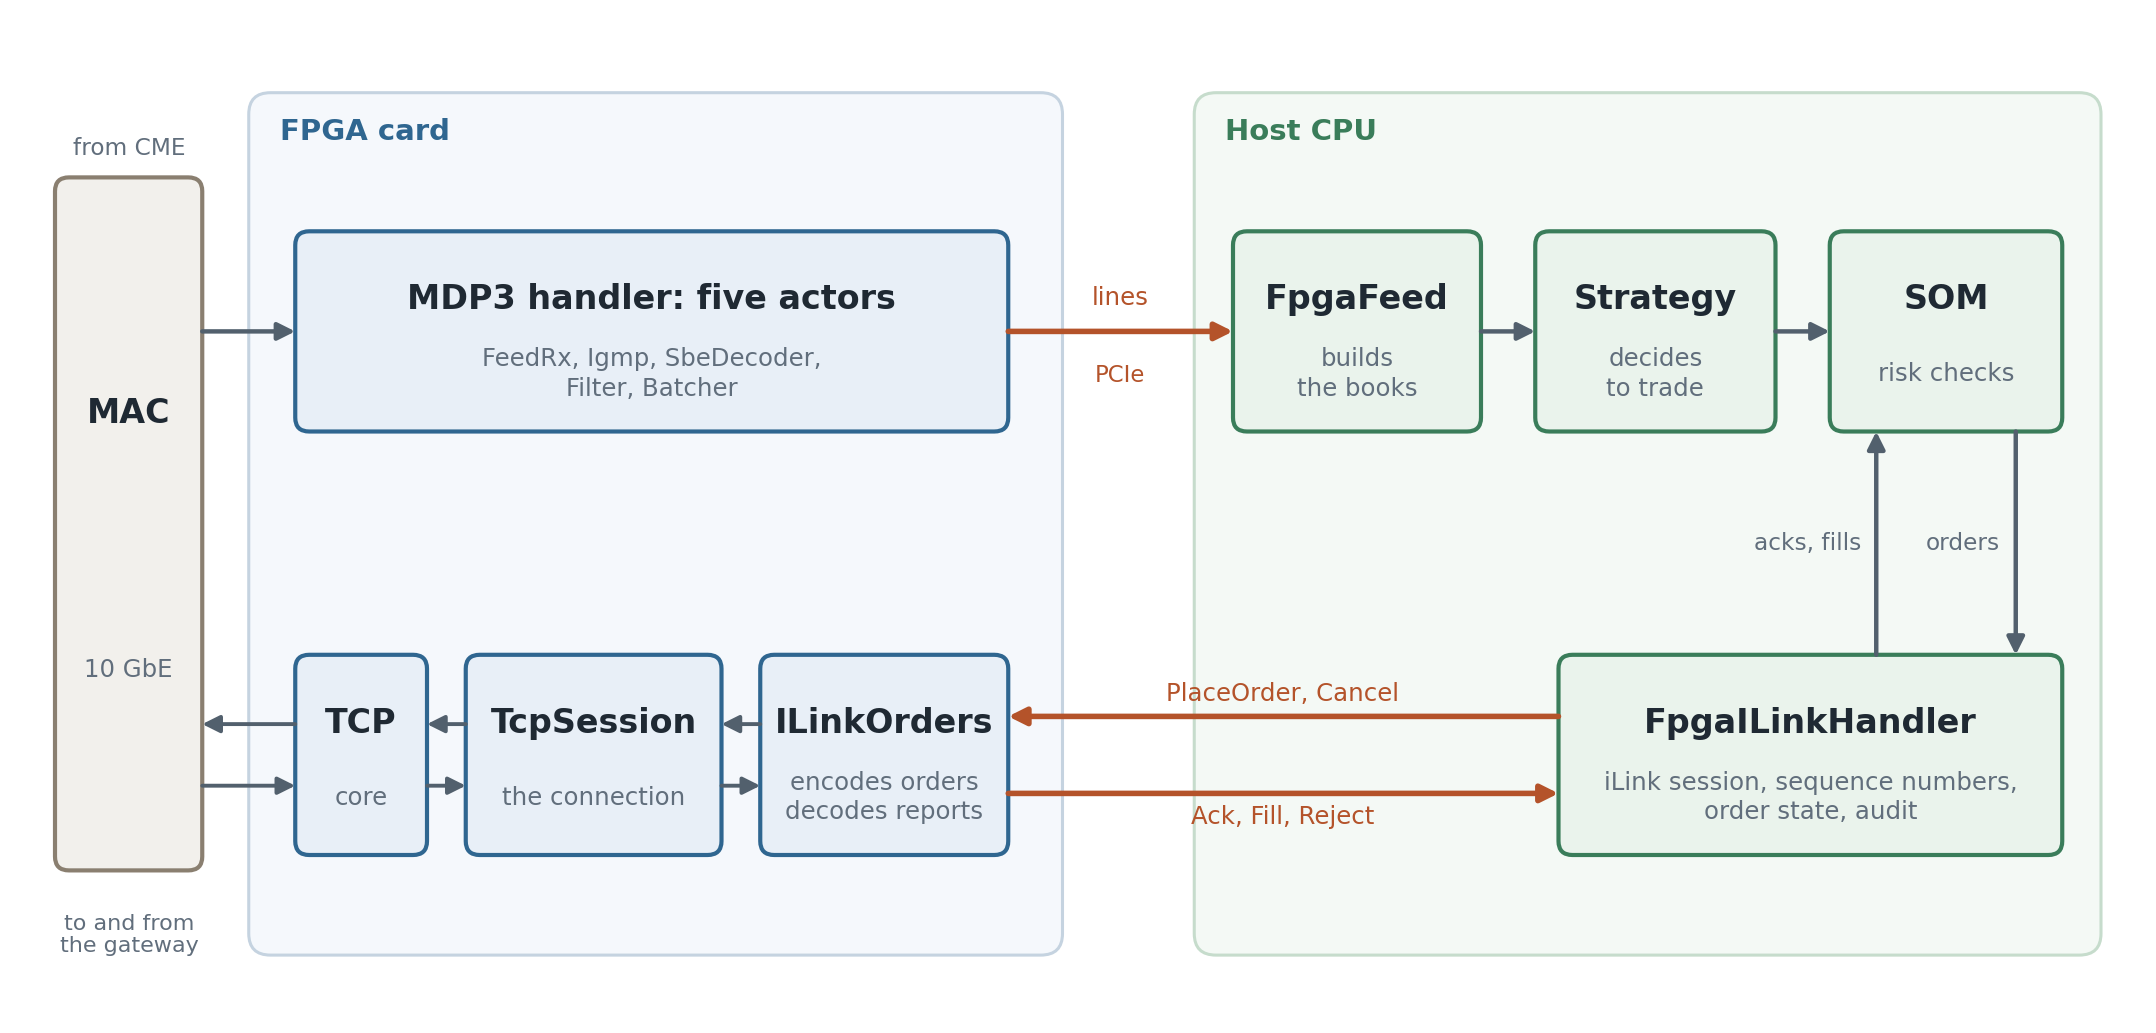
\includegraphics[width=\textwidth]{hybrid.png}
\caption{The full hybrid trading system. Both protocol ends, MDP3 in and
iLink~3 out, are actors on the card; the books, the strategy, the risk checks
and the iLink session are actors on the CPU. The thick arrows cross PCIe.}
\label{fig:hybrid}
\end{figure}

\begin{table}[h]
\centering
\caption{Where each part of the trading path runs in the hybrid system, and
why.}
\label{tab:placement}
\small
\begin{tabular}{p{4.3cm} p{1.3cm} p{7.4cm}}
\toprule
Part & Where & Why \\
\midrule
Ethernet, IP, UDP; multicast join & card & per byte; the port belongs to the FPGA \\
SBE decode, filter, packing & card & per byte, and the source of the software tail \\
Books & CPU & one per security, and read by the strategy, which is on the CPU \\
Strategy & CPU & the decision; the actors are those of today \\
Risk checks (SOM) & CPU & every order passes them; unchanged \\
iLink session, sequence numbers, order state, audit & CPU & state, and every decision to send; no state shared with the card \\
SBE encode of orders, decode of reports & card & per message, proportional to its bytes \\
TCP & card & a third-party engine, owned by an actor \\
\bottomrule
\end{tabular}
\end{table}

The division follows one rule: the card does the work that is proportional to
bytes on the wire and needs no decision, and the CPU keeps state, decisions and
risk. The rule puts the boundary where little crosses, as
Section~\ref{sec:boundary} recommends: the wanted events, three to a 64-byte
line, from the card; one message per order to the card; one message per
acknowledgement or fill from it. Both halves fit on the card's device with room
to spare: the MDP3 handler uses 0.6\% of its LUTs, and the commercial TCP
engine is quoted at about 3\%.

\subsection{Threads on the CPU}

Two CPU actors receive from the card, FpgaFeed and FpgaILinkHandler, and both
therefore have lane mailboxes and spin. The CPU framework allows them, with the
strategy and SOM, to be placed in one group, so that the path from book update
to order runs on one thread through \fs{} calls, and the one loop of the group's
mailbox polls both sets of lanes. That is the one-thread placement which, in the companion paper's study of the
software market-data path, had the lower latency \cite{fastsend}; whether it is also the best placement here, with the decode
moved off the CPU, is a measurement still to be made.

\subsection{The tick-to-trade path}

From a packet on the wire to an order on the wire, the path is: the packet
arrives and is decoded on the card; its last line crosses PCIe to host memory;
FpgaFeed applies the last events; the strategy, SOM and FpgaILinkHandler run on
the CPU; the order crosses PCIe to the card; ILinkOrders encodes it and the TCP
engine sends it. Of these, the market-data half has the estimates of
Section~\ref{sec:budget}: about 100~ns on the card after the packet's last byte
and about 300--400~ns across PCIe. The CPU's part is the same strategy and risk
code that runs today, and the order half has no figures yet. We give no
tick-to-trade number.

What the design does establish is the shape of the path. Nothing on it grows
with the length of the incoming packet after its last byte; nothing on it reads
across the bus; no thread hands a message to another; and it crosses PCIe
twice, once in each direction. Those two crossings are now the largest fixed
costs that are not the CPU's own work, and removing them means moving the
decision itself onto the card --- a book and a simple signal on the FPGA ---
which raises the question of how risk checks are kept on a path that no longer
passes through the CPU. We leave that question open.

\subsection{One system, three deployments}

Because the card's actors and the software components they replace accept and
produce the same messages, the hybrid system is a deployment of kaspar-hft, not
a second system. The same strategy and SOM run in three configurations: in
backtest, from recorded packets through the software handler, with simulated
order entry; in production on the CPU alone, with the software market-data
handler and iLink handler; and in production with the card, with FpgaFeed and
FpgaILinkHandler in their place. The companion paper's production/simulation
duality \cite{fastsend} survives the card: a strategy is still developed and
tested without one.

% ---------------------------------------------------------------
\section{Software and hardware: a duality of the actor}
\label{sec:duality}
% ---------------------------------------------------------------

The companion paper observed that a group sharing one queue is at once a
real-time engine and a deterministic simulator: the same actors run in
production on live input and in backtest on recorded input
\cite{fastsend}. The FPGA framework has an analogue one level down. The same
actor source is compiled twice: by HLS into a circuit, and by an ordinary C++
compiler into a model in which each process's step is called once per
simulated clock. The model is deterministic, runs a full trading session in
minutes rather than the days RTL simulation would take, and exercises exactly
the handlers that the circuit will run. The results of
Section~\ref{sec:results} were obtained that way, and RTL co-simulation then
confirmed on a slice of the session that the circuit computes the same thing.

The duality has a limit the CPU one does not: the model has no pipeline
latency and no timing, so it establishes behaviour and bounds in clocks, not
nanoseconds; and it cannot detect constructs that HLS will reject or
mis-synthesize (Table~\ref{tab:rules}). Both are left to synthesis and
co-simulation, which is why every design passes all four levels of
Section~\ref{sec:verify}.

% ---------------------------------------------------------------
\section{Discussion and limitations}
\label{sec:disc}
% ---------------------------------------------------------------

\paragraph{The model is narrower on the card.} One actor of each type per
design; at most four sends per handler; message payloads of 48 bytes of
integers; no \fs{} between processes or across PCIe; queues sized at build
time, and a group's own queue that drops when full rather than stalling. Each is
a consequence of fixed hardware and is checked, in software builds at least,
rather than silently tolerated.

% ---------------------------------------------------------------
\section{Future work}
\label{sec:future}
% ---------------------------------------------------------------

\begin{enumerate}[leftmargin=1.6em]
  \item \textbf{The card.} The MAC and clock-domain crossings, the frame check
  verdict carried to the End line, and the PCIe DMA engine with its windows and
  lanes; then a measurement of wire-to-book latency on hardware.
  \item \textbf{Measured card latency in co-simulation}, replacing the
  estimate of Section~\ref{sec:results}.
  \item \textbf{Several actors of one type} in a design, and pipelined groups
  whose handlers loop.
  \item \textbf{Market-by-order data} through the card, passed to the CPU's
  order-by-order book as market-by-price data is now; more channels; A/B feed
  arbitration.
  \item \textbf{Order entry on the card,} the phases of
  Section~\ref{sec:ilink}, beginning with a measurement of today's order path;
  then the full system of Section~\ref{sec:fullsystem}, and its tick-to-trade
  latency on hardware.
  \item \textbf{The trigger on the card,} with a book on the card, so that a
  simple signal acts without crossing PCIe.
\end{enumerate}

% ---------------------------------------------------------------
\section{Conclusion}
% ---------------------------------------------------------------

The actor model can cross the PCIe slot. On the FPGA, a process becomes an
always-running hardware task that takes one message per clock, a \snd{} becomes
one write into a FIFO, a group shares one process with \fs{} as an inline call
confined to the group, and the pointers on which the CPU framework rests become
port numbers, outboxes and one object per actor type, all fixed when the design
is built. Across the bus, CPU and FPGA actors exchange the same 64-byte messages
through rings in which each side writes only across the bus and reads only its
own memory, the receiving thread's own mailbox polls the card, and neither
side's handlers depend on where their peers run. What an actor's author writes
does not change.

The market-data handler shows what that buys. Built from five actors on the
card and one on the CPU, it decodes, filters and packs each packet as it
arrives, and the CPU builds the books line by line while the packet is still on
the wire. Over a full CME session, the card's work after a packet's last byte
never grew with the packet, which is the property a software handler lacks and
the source of its tail. On the card's device the design meets 250~MHz with every
stage at one step per clock, in under 1\% of the chip. The remaining latency is
dominated by the bus. The same rule --- the card takes the work proportional to
bytes on the wire, the CPU keeps state, decisions and risk --- places order
entry and gives the full hybrid system, in which both protocol ends are actors
on the card and the strategy is unchanged, whether it runs in backtest, on the
CPU alone, or with the card. What remains to be shown is that system on
hardware.

% ---------------------------------------------------------------
\begin{thebibliography}{99}
% ---------------------------------------------------------------
\bibitem{fastsend} V.~Maciejewski.
  \emph{Adapting the Actor Model of Concurrency for High-Frequency Trading:
  Synchronous Message Delivery (\texttt{fast\_send}) and a Tick-to-Book Latency
  Study.} arXiv:2609.21173, 2026. \url{https://arxiv.org/abs/2609.21173}.
\bibitem{mdarrival} V.~Maciejewski.
  \emph{The Market-Data Arrival Process is Self-Exciting: Bursts, Packet
  Coalescing, and the Socket-to-Book Latency Tail.} kaspar-hft technical report
  (in preparation), 2026.
\bibitem{hewitt1973} C.~Hewitt, P.~Bishop, and R.~Steiger.
  \emph{A Universal Modular ACTOR Formalism for Artificial Intelligence.}
  Proc.\ 3rd International Joint Conference on Artificial Intelligence (IJCAI),
  1973.
\bibitem{agha1986} G.~Agha.
  \emph{Actors: A Model of Concurrent Computation in Distributed Systems.}
  MIT Press, 1986.
\bibitem{kahn1974} G.~Kahn.
  \emph{The Semantics of a Simple Language for Parallel Programming.}
  Proc.\ IFIP Congress 74, North-Holland, 1974.
\bibitem{lee1987sdf} E.~A.~Lee and D.~G.~Messerschmitt.
  \emph{Synchronous Data Flow.} Proceedings of the IEEE, 75(9), 1987.
\bibitem{cal2003} J.~Eker and J.~W.~Janneck.
  \emph{CAL Language Report: Specification of the CAL Actor Language.}
  Technical Report UCB/ERL M03/48, University of California, Berkeley, 2003.
\bibitem{streamblocks2020} E.~Bezati, M.~Emami, and J.~R.~Larus.
  \emph{Advanced Dataflow Programming using Actor Machines for High-Level
  Synthesis.} Proc.\ ACM/SIGDA International Symposium on Field-Programmable
  Gate Arrays (FPGA), 2020. \url{https://doi.org/10.1145/3373087.3375330}.
\bibitem{streamblocks2021} E.~Bezati, M.~Emami, J.~W.~Janneck, and
  J.~R.~Larus. \emph{StreamBlocks: A Compiler for Heterogeneous Dataflow
  Computing (Technical Report).} arXiv:2107.09333, 2021.
\bibitem{reconos2009} E.~L\"ubbers and M.~Platzner.
  \emph{ReconOS: Multithreaded Programming for Reconfigurable Computers.}
  ACM Transactions on Embedded Computing Systems, 9(1), 2009.
  \url{https://doi.org/10.1145/1596532.1596540}.
\bibitem{coyote2020} D.~Korolija, T.~Roscoe, and G.~Alonso.
  \emph{Do OS Abstractions Make Sense on FPGAs?} Proc.\ 14th USENIX Symposium
  on Operating Systems Design and Implementation (OSDI), 2020.
\bibitem{orcc2013} H.~Yviquel, A.~Lorence, K.~Jerbi, G.~Cocherel, A.~Sanchez,
  and M.~Raulet. \emph{Orcc: Multimedia Development Made Easy.} Proc.\ 21st ACM
  International Conference on Multimedia, pp.~863--866, 2013.
  \url{https://doi.org/10.1145/2502081.2502231}.
\bibitem{xronos2013} E.~Bezati, M.~Mattavelli, and J.~W.~Janneck.
  \emph{High-Level Synthesis of Dataflow Programs for Signal Processing
  Systems.} Proc.\ 8th International Symposium on Image and Signal Processing
  and Analysis (ISPA), pp.~750--754, 2013.
  \url{https://doi.org/10.1109/ISPA.2013.6703837}.
\bibitem{caph2011} J.~S\'erot, F.~Berry, and S.~Ahmed.
  \emph{Implementing Stream-Processing Applications on FPGAs: A DSL-Based
  Approach.} Proc.\ 21st International Conference on Field Programmable Logic
  and Applications (FPL), pp.~130--137, 2011.
  \url{https://doi.org/10.1109/FPL.2011.32}.
\bibitem{lee2003actororiented} E.~A.~Lee, S.~Neuendorffer, and M.~J.~Wirthlin.
  \emph{Actor-Oriented Design of Embedded Hardware and Software Systems.}
  Journal of Circuits, Systems and Computers, 12(3):231--260, 2003.
  \url{https://doi.org/10.1142/S0218126603000751}.
\bibitem{ptolemyvhdl2008} M.-K.~Leung, T.~E.~Filiba, and V.~Nagpal.
  \emph{VHDL Code Generation in the Ptolemy II Environment.} Technical Report
  UCB/EECS-2008-140, University of California, Berkeley, 2008.
\bibitem{tmdmpi2006} M.~Salda\~na and P.~Chow. \emph{TMD-MPI: An MPI
  Implementation for Multiple Processors Across Multiple FPGAs.} Proc.\ 16th
  International Conference on Field Programmable Logic and Applications (FPL),
  2006. \url{https://doi.org/10.1109/FPL.2006.311233}.
\bibitem{tmdmpi2006hw} M.~Salda\~na, D.~Nunes, E.~Ramalho, and P.~Chow.
  \emph{Configuration and Programming of Heterogeneous Multiprocessors on a
  Multi-FPGA System Using TMD-MPI.} Proc.\ IEEE International Conference on
  Reconfigurable Computing and FPGAs (ReConFig), 2006.
  \url{https://doi.org/10.1109/RECONF.2006.307779}.
\bibitem{tmdmpi2010} M.~Salda\~na, A.~Patel, C.~Madill, D.~Nunes, D.~Wang,
  P.~Chow, R.~Wittig, H.~Styles, and A.~Putnam. \emph{MPI as a Programming
  Model for High-Performance Reconfigurable Computers.} ACM Transactions on
  Reconfigurable Technology and Systems, 3(4), 2010.
  \url{https://doi.org/10.1145/1862648.1862652}.
\bibitem{galapagos2018} N.~Tarafdar, N.~Eskandari, V.~Sharma, C.~Lo, and
  P.~Chow. \emph{Galapagos: A Full Stack Approach to FPGA Integration in the
  Cloud.} IEEE Micro, 38(6):18--24, 2018.
  \url{https://doi.org/10.1109/MM.2018.2877290}.
\bibitem{galapagos2019} N.~Eskandari, N.~Tarafdar, D.~Ly-Ma, and P.~Chow.
  \emph{A Modular Heterogeneous Stack for Deploying FPGAs and CPUs in the Data
  Center.} Proc.\ ACM/SIGDA International Symposium on Field-Programmable Gate
  Arrays (FPGA), pp.~262--271, 2019.
  \url{https://doi.org/10.1145/3289602.3293909}.
\bibitem{shoal2021} V.~Sharma and P.~Chow. \emph{Exploring PGAS Communication
  for Heterogeneous Clusters with FPGAs.} Proc.\ ACM/SIGDA International
  Symposium on Field-Programmable Gate Arrays (FPGA), 2021; extended version
  arXiv:2104.12350. \url{https://doi.org/10.1145/3431920.3439469}.
\bibitem{lime2010} J.~Auerbach, D.~F.~Bacon, P.~Cheng, and R.~Rabbah.
  \emph{Lime: A Java-Compatible and Synthesizable Language for Heterogeneous
  Architectures.} Proc.\ ACM International Conference on Object-Oriented
  Programming Systems, Languages and Applications (OOPSLA), pp.~89--108, 2010.
  \url{https://doi.org/10.1145/1869459.1869469}.
\bibitem{kiwi2008} S.~Singh and D.~J.~Greaves. \emph{Kiwi: Synthesis of FPGA
  Circuits from Parallel Programs.} Proc.\ 16th IEEE Symposium on
  Field-Programmable Custom Computing Machines (FCCM), pp.~3--12, 2008.
  \url{https://doi.org/10.1109/FCCM.2008.46}.
\bibitem{legup2013} J.~Choi, S.~Brown, and J.~Anderson. \emph{From Software
  Threads to Parallel Hardware in High-Level Synthesis for FPGAs.} Proc.\
  International Conference on Field-Programmable Technology (FPT),
  pp.~270--277, 2013. \url{https://doi.org/10.1109/FPT.2013.6718365}.
\bibitem{hthreads2008} D.~Andrews, R.~Sass, E.~Anderson, J.~Agron, W.~Peck,
  J.~Stevens, F.~Baijot, and E.~Komp. \emph{Achieving Programming Model
  Abstractions for Reconfigurable Computing.} IEEE Transactions on Very Large
  Scale Integration (VLSI) Systems, 16(1):34--44, 2008.
  \url{https://doi.org/10.1109/TVLSI.2007.912106}.
\bibitem{borph2008} H.~K.-H.~So and R.~Brodersen. \emph{A Unified
  Hardware/Software Runtime Environment for FPGA-Based Reconfigurable Computers
  Using BORPH.} ACM Transactions on Embedded Computing Systems, 7(2), 2008.
  \url{https://doi.org/10.1145/1331331.1331338}.
\bibitem{clicknp2016} B.~Li, K.~Tan, L.~Luo, Y.~Peng, R.~Luo, N.~Xu,
  Y.~Xiong, P.~Cheng, and E.~Chen. \emph{ClickNP: Highly Flexible and High
  Performance Network Processing with Reconfigurable Hardware.} Proc.\ ACM
  SIGCOMM, pp.~1--14, 2016. \url{https://doi.org/10.1145/2934872.2934897}.
\bibitem{erlanghls2016} H.~Takebayashi, N.~Ishiura, K.~Azuma, N.~Yoshida, and
  H.~Kanbara. \emph{High-Level Synthesis of Embedded Systems Controller from
  Erlang.} Proc.\ 20th Workshop on Synthesis And System Integration of Mixed
  Information Technologies (SASIMI), 2016.
\bibitem{erlanghls2017} K.~Azuma, N.~Ishiura, N.~Yoshida, and H.~Kanbara.
  \emph{Distributed Memory Architecture for High-Level Synthesis of Embedded
  Controllers from Erlang.} Proc.\ 16th ACM SIGPLAN International Workshop on
  Erlang, pp.~13--19, 2017. \url{https://doi.org/10.1145/3123569.3123574}.
\bibitem{cafopencl2015} R.~Hiesgen, D.~Charousset, and T.~C.~Schmidt.
  \emph{Manyfold Actors: Extending the C++ Actor Framework to Heterogeneous
  Many-Core Machines Using OpenCL.} Proc.\ 5th International Workshop on
  Programming Based on Actors, Agents, and Decentralized Control (AGERE),
  pp.~45--56, 2015. \url{https://doi.org/10.1145/2824815.2824820}.
\bibitem{morris2009} G.~W.~Morris, D.~B.~Thomas, and W.~Luk.
  \emph{FPGA Accelerated Low-Latency Market Data Feed Processing.}
  Proc.\ 17th IEEE Symposium on High Performance Interconnects (HOTI), 2009.
\bibitem{litz2011} H.~Litz, C.~Leber, and B.~Geib.
  \emph{DSL Programmable Engine for High Frequency Trading Acceleration.}
  Proc.\ 4th Workshop on High Performance Computational Finance (WHPCF), 2011.
\bibitem{lockwood2012} J.~W.~Lockwood, A.~Gupte, N.~Mehta, M.~Blott,
  T.~English, and K.~Vissers.
  \emph{A Low-Latency Library in FPGA Hardware for High-Frequency Trading
  (HFT).} Proc.\ 20th IEEE Symposium on High-Performance Interconnects (HOTI),
  2012, pp.~9--16.
\bibitem{ug1399} AMD.
  \emph{Vitis High-Level Synthesis User Guide (UG1399).} 2026.
  \url{https://docs.amd.com/r/en-US/ug1399-vitis-hls}.
\bibitem{ug1523} AMD.
  \emph{Alveo X3522 User Guide (UG1523).}
  \url{https://docs.amd.com/r/en-US/ug1523-x3522-user}.
\bibitem{pg210} AMD.
  \emph{10G/25G High Speed Ethernet Subsystem Product Guide (PG210).}
\bibitem{rfc2236} W.~Fenner.
  \emph{Internet Group Management Protocol, Version 2.} RFC 2236, IETF, 1997.
\bibitem{fixsbe} FIX Trading Community.
  \emph{Simple Binary Encoding (SBE), Version 1.0.} Technical Standard, 2020.
  \url{https://www.fixtrading.org/standards/sbe/}.
\bibitem{cmemdp3} CME Group.
  \emph{CME MDP 3.0 Market Data.} CME Client Systems Wiki.
\bibitem{orthogone2023} Orthogone Technologies.
  \emph{Orthogone Technologies Unveils FPGA-Based Lightning-Fast PCIe DMA
  Controller Solution.} Press release and product brief, 2023.
  \url{https://prnewswire.com/news-releases/orthogone-technologies-unveils-fpga-based-lightning-fast-pcie-dma-controller-solution-301953564.html}.
\bibitem{cmeilink3} CME Group.
  \emph{iLink 3 Binary Order Entry.} CME Client Systems Wiki.
\bibitem{sidler2015} D.~Sidler, G.~Alonso, M.~Blott, K.~Karras, K.~Vissers,
  and R.~Carley. \emph{Scalable 10Gbps TCP/IP Stack Architecture for
  Reconfigurable Hardware.} Proc.\ IEEE 23rd Annual International Symposium on
  Field-Programmable Custom Computing Machines (FCCM), 2015, pp.~36--43.
  \url{https://doi.org/10.1109/FCCM.2015.12}.
\bibitem{fpgastack} Systems Group, ETH Zurich.
  \emph{fpga-network-stack: a TCP/IP, RoCEv2 and UDP/IP stack for FPGAs.}
  \url{https://github.com/fpgasystems/fpga-network-stack}, accessed 2026.
\bibitem{npap} Missing Link Electronics.
  \emph{NPAP: TCP/UDP/IP Network Protocol Accelerator Platform, 100G on AMD
  Alveo.} Product brief, 2026.
  \url{https://www.missinglinkelectronics.com/wp-content/uploads/2026/03/MLE-NPAP-100G-on-AMD-Alveo-20260228.pdf}.
\end{thebibliography}

\end{document}
